%%%%%%%%%%%%%%%%%%%%%%%%%%%%%%%%%%%%%%%%%
% Masters/Doctoral Thesis 
% LaTeX Template
% Version 2.4 (22/11/16)
%
% This template has been downloaded from:
% http://www.LaTeXTemplates.com
%
% Version 2.x major modifications by:
% Vel (vel@latextemplates.com)
%
% This template is based on a template by:
% Steve Gunn (http://users.ecs.soton.ac.uk/srg/softwaretools/document/templates/)
% Sunil Patel (http://www.sunilpatel.co.uk/thesis-template/)
%
% Template license:
% CC BY-NC-SA 3.0 (http://creativecommons.org/licenses/by-nc-sa/3.0/)
%
%%%%%%%%%%%%%%%%%%%%%%%%%%%%%%%%%%%%%%%%%

%----------------------------------------------------------------------------------------
%	PACKAGES AND OTHER DOCUMENT CONFIGURATIONS
%----------------------------------------------------------------------------------------

\documentclass[
11pt, % The default document font size, options: 10pt, 11pt, 12pt
%oneside, % Two side (alternating margins) for binding by default, uncomment to switch to one side
english, % ngerman for German
singlespacing, % Single line spacing, alternatives: onehalfspacing or doublespacing
%draft, % Uncomment to enable draft mode (no pictures, no links, overfull hboxes indicated)
%nolistspacing, % If the document is onehalfspacing or doublespacing, uncomment this to set spacing in lists to single
%liststotoc, % Uncomment to add the list of figures/tables/etc to the table of contents
%toctotoc, % Uncomment to add the main table of contents to the table of contents
%parskip, % Uncomment to add space between paragraphs
%nohyperref, % Uncomment to not load the hyperref package
headsepline, % Uncomment to get a line under the header
chapterinoneline, % Uncomment to place the chapter title next to the number on one line
%consistentlayout, % Uncomment to change the layout of the declaration, abstract and acknowledgements pages to match the default layout
]{MastersDoctoralThesis} % The class file specifying the document structure

\usepackage[utf8]{inputenc} % Required for inputting international characters
\usepackage[T1]{fontenc} % Output font encoding for international characters

\usepackage{lmodern} % Use the Palatino font by default

\usepackage[backend=bibtex,style=numeric,natbib=true]{biblatex} % Use the bibtex backend with the authoryear citation style (which resembles APA)

\addbibresource{thesis-articles.bib} % The filename of the bibliography

\usepackage[autostyle=true]{csquotes} % Required to generate language-dependent quotes in the bibliography

% Elliott-added packages
\usepackage{amsmath} % for align and other environments
\usepackage{listings}
\usepackage{float}   % for H figure specifier
\usepackage{indentfirst} % to indent after sections

%----------------------------------------------------------------------------------------
%	MARGIN SETTINGS
%----------------------------------------------------------------------------------------

\geometry{
	paper=a4paper, % Change to letterpaper for US letter
	inner=2.5cm, % Inner margin
	outer=2.5cm, % Outer margin
	bindingoffset=.0cm, % Binding offset
	top=1.5cm, % Top margin
	bottom=1.5cm, % Bottom margin
	%showframe, % Uncomment to show how the type block is set on the page
}

%----------------------------------------------------------------------------------------
%	THESIS INFORMATION
%----------------------------------------------------------------------------------------

\thesistitle{Simulating dynein'’s powerstroke using Brownian dynamics} % Your thesis title, this is used in the title and abstract, print it elsewhere with \ttitle
\supervisor{Dr. David \textsc{Roundy}} % Your supervisor's name, this is used in the title page, print it elsewhere with \supname
\examiner{} % Your examiner's name, this is not currently used anywhere in the template, print it elsewhere with \examname
\degree{Bachelor of Science} % Your degree name, this is used in the title page and abstract, print it elsewhere with \degreename
\author{Elliott \textsc{Capek}} % Your name, this is used in the title page and abstract, print it elsewhere with \authorname
\addresses{} % Your address, this is not currently used anywhere in the template, print it elsewhere with \addressname

\subject{Physics} % Your subject area, this is not currently used anywhere in the template, print it elsewhere with \subjectname
\keywords{} % Keywords for your thesis, this is not currently used anywhere in the template, print it elsewhere with \keywordnames
\university{\href{http://www.university.com}{Oregon State University}} % Your university's name and URL, this is used in the title page and abstract, print it elsewhere with \univname
\department{\href{http://physics.oregonstate.edu}{Oregon State University Department of Physics}} % Your department's name and URL, this is used in the title page and abstract, print it elsewhere with \deptname
\group{\href{http://physics.oregonstate.edu/~roundyd/}{Roundy Research Group}} % Your research group's name and URL, this is used in the title page, print it elsewhere with \groupname
\faculty{} % Your faculty's name and URL, this is used in the title page and abstract, print it elsewhere with \facname

\AtBeginDocument{
\hypersetup{pdftitle=\ttitle} % Set the PDF's title to your title
\hypersetup{pdfauthor=\authorname} % Set the PDF's author to your name
\hypersetup{pdfkeywords=\keywordnames} % Set the PDF's keywords to your keywords
}

\begin{document}

\frontmatter % Use roman page numbering style (i, ii, iii, iv...) for the pre-content pages

\pagestyle{plain} % Default to the plain heading style until the thesis style is called for the body content

%----------------------------------------------------------------------------------------
%	TITLE PAGE
%----------------------------------------------------------------------------------------

\begin{titlepage}
\begin{center}

\vspace*{.06\textheight}
{\scshape\LARGE \univname\par}\vspace{1.5cm} % University name
\textsc{\Large Undergraduate Thesis}\\[0.5cm] % Thesis type

\HRule \\[0.4cm] % Horizontal line
{\huge \bfseries \ttitle\par}\vspace{0.4cm} % Thesis title
\HRule \\[1.5cm] % Horizontal line
 
\begin{minipage}[t]{0.4\textwidth}
\begin{flushleft} \large
\emph{Author:}\\
{\authorname} % Author name - remove the \href bracket to remove the link
\end{flushleft}
\end{minipage}
\begin{minipage}[t]{0.4\textwidth}
\begin{flushright} \large
\emph{Supervisor:} \\
{\supname} % Supervisor name - remove the \href bracket to remove the link  
\end{flushright}
\end{minipage}\\[3cm]
 
\vfill

\large \textit{A thesis submitted in fulfillment of the requirements\\ for the degree of \degreename}\\[0.3cm] % University requirement text
\textit{in the}\\[0.4cm]
\groupname\\\deptname\\[2cm] % Research group name and department name
 
\vfill

{\large \today}\\[4cm] % Date
%\includegraphics{Logo} % University/department logo - uncomment to place it
 
\vfill
\end{center}
\end{titlepage}

%----------------------------------------------------------------------------------------
%	ABSTRACT PAGE
%----------------------------------------------------------------------------------------

\begin{abstract}
\addchaptertocentry{\abstractname} % Add the abstract to the table of contents
Dynein is a motor protein which transports cargo along tracks inside the cell. Like related motor proteins kinesin and myosin, dynein uses cellular energy to take steps with its two foot domains. Unlike kinesin or myosin, dynein's stepping pattern is highly varied: it can take steps between zero and 60nm in both the forwards and backwards directions. It is believed that dynein takes such broad, stochastic steps because its large size and several elastic regions make it more influenced by Brownian motion. To test this, we model the motor as a 2D system of elastic hinges, then simulate this model using Brownian dynamics. Preliminary results indicate such a model is capable of taking steps between zero and 25nm. These results give hope that, with further tweaking, the model may be able to generate both larger steps and backwards steps.
\end{abstract}
\newpage

%% %----------------------------------------------------------------------------------------
%% %	ACKNOWLEDGEMENTS
%% %----------------------------------------------------------------------------------------

%% \begin{acknowledgements}
%% \addchaptertocentry{\acknowledgementname} % Add the acknowledgements to the table of contents
%% The acknowledgments and the people to thank go here, don't forget to include your project advisor\ldots
%% \end{acknowledgements}

%----------------------------------------------------------------------------------------
%	LIST OF CONTENTS/FIGURES/TABLES PAGES
%----------------------------------------------------------------------------------------

\tableofcontents % Prints the main table of contents
\newpage

\listoffigures % Prints the list of figures
\newpage

%% \listoftables % Prints the list of tables
\newpage

%% %----------------------------------------------------------------------------------------
%% %	ABBREVIATIONS
%% %----------------------------------------------------------------------------------------

%% \begin{abbreviations}{ll} % Include a list of abbreviations (a table of two columns)

%% \textbf{MT} & \textbf{M}icro\textbf{t}ubule\\
%% \textbf{MTBD} & \textbf{M}icro\textbf{t}ubule \textbf{B}inding \textbf{D}omain\\

%% \end{abbreviations}

%% %----------------------------------------------------------------------------------------
%% %	PHYSICAL CONSTANTS/OTHER DEFINITIONS
%% %----------------------------------------------------------------------------------------

%% \begin{constants}{lr@{${}={}$}l} % The list of physical constants is a three column table

%% % The \SI{}{} command is provided by the siunitx package, see its documentation for instructions on how to use it

%% Speed of Light & $c_{0}$ & \SI{2.99792458e8}{\meter\per\second} (exact)\\
%% %Constant Name & $Symbol$ & $Constant Value$ with units\\

%% \end{constants}

%% %----------------------------------------------------------------------------------------
%% %	SYMBOLS
%% %----------------------------------------------------------------------------------------

%% \begin{symbols}{lll} % Include a list of Symbols (a three column table)

%% $a$ & distance & \si{\meter} \\
%% $P$ & power & \si{\watt} (\si{\joule\per\second}) \\
%% %Symbol & Name & Unit \\

%% \addlinespace % Gap to separate the Roman symbols from the Greek

%% $\omega$ & angular frequency & \si{\radian} \\

%% \end{symbols}

%% %----------------------------------------------------------------------------------------
%% %	DEDICATION
%% %----------------------------------------------------------------------------------------

%% \dedicatory{For/Dedicated to/To my\ldots} 

%----------------------------------------------------------------------------------------
%	THESIS CONTENT - CHAPTERS
%----------------------------------------------------------------------------------------

\mainmatter % Begin numeric (1,2,3...) page numbering

\pagestyle{thesis} % Return the page headers back to the "thesis" style

% Include the chapters of the thesis as separate files from the Chapters folder
% Uncomment the lines as you write the chapters

%----------------------------------------------------------------------------------------
%	THESIS CONTENT - CHAPTERS
%----------------------------------------------------------------------------------------
\chapter{Introduction}
\label{chap:Introduction}

\blockquote{An embryo in its spherical blastula stage has spherical symmetry [...]. But a system which has spherical symmetry, and whose state is changing because of chemical reactions and diffusion, will remain spherically symmetrical for ever [...]. It certainly cannot result in an organism such as a horse, which is not spherically symmetrical. \textbf{Alan Turing, The Chemical Basis of Morphogenesis, 1952}}

Cells need to create asymmetric, heterogeneous structures inside themselves in order to function. However, diffusive processes cannot create this asymmetry. How then do cells create the heterogeneous structures they need to exist? Motor proteins are part of the answer. Motor proteins are structures which use energy to create directed motion in cells. In broad terms, they are mechanical creators of asymmetry. This thesis explores a hypothesis about how one such motor protein, dynein, generates directed motion.\\

\section{Motivation}
Motor proteins are cellular structures which use chemical energy to do work and generate motion. Kinesin, myosin and dynein are the three main motor proteins in cells. Though these proteins have significantly different ancestors \cite{hook-family}, they all evolved into a single similar structure. In biology when a structure is evolved three separate times, it is a sign that nature has found an efficient way of solving a problem. How, then, do motor proteins work?\\

The basic process is simple. Kinesin, myosin and dynein each use two binding domains to attach to a surface. These binding domains are connected via a linker domain. Each motor protein is an engine which undergoes cycles, where each cycle moves the motor across a surface. In a single cycle a binding domain unbinds from a surface, tenses its foot to kick forward, rebinds, then untenses its foot to pull the whole motor forward. This pattern is repeated by both feet to generate motion \cite{kinesin-cycle, myosin-cycle}.\\

Although the three motor protein families operate using the same stepping cycle, their behaviors differ significantly. Kinesin and myosin are predictable motors which step in the forward direction with a regular step size. In contrast, dynein's stepping pattern varies in both size and direction. The motor can take 64nm steps forward or 32nm steps backward, and often steps sideways as well \cite{weihongpaper}. How can motors which implement the same release, lever, bind, lurch stepping mechanism behave so differently?\\

One possibility is that dynein's size and organization are responsible for the motor's odd stepping pattern. Dynein is much larger than kinesin or myosin, so its feet may need to move significantly further during each cycle. Due to the random nature of Brownian motion from water particle collisions, there may be significantly more variance in the path taken by dynein's feet compared to other motor feet. This could explain the large variance in step size. Another contributing factor could be that dynein is so large that it can twist and contort during its step, allowing varying and even backwards steps, which a small motor would be too stiff to achieve.\\

This thesis describes an experiment which aims to test whether Brownian motion and flexibility cause dynein's unique stepping pattern. To do this, we construct a mathematical model of the dynein motor which exhibits flexibility and feels Brownian forces. We then simulate the model and compare its behavior to real dynein.\\

%% Dynein:
%% feet which bind to track
%% motor connected to feet which generates the force
%% -----------
%% ATP binding causes dissociation
%% Also causes forward kick
%% ATP hydrolysis
%% rebinding causes ADP rejection and forward lurch
%% restart

%% Kinesin:
%% feet which bind to track
%% connected via lever arm to cargo binding domain
%% -----------
%% ATP binding causes forward kick
%% ATP hydrolysis
%% MT binding, ADP, Pi rejection
%% Other foot unbinds

%% Myosin:
%% Feet which bind to track
%% connected via lever arm to cargo binding domain
%% ----------
%% actin binding causes Pi rejection, strengthening binding
%% binding causes foot to change relative to lever, shifting the motor forward
%% ATP binding causes dissocaition and undoing the powerstroke

\section{What is dynein?}
\subsection{Basics}
Dynein is a cellular structure which converts chemical energy to mechanical energy. It does so by reacting with adenosine triphosphate (ATP) to take steps along long cellular tracks known as microtubules (MTs). Dynein's mechanical energy is used for various cellular functions, including to transport molecules around the cell, pull chromosomes during division, and move cellular propellers known as cilia \cite{cianfroccoreview}.\\

Dynein is a protein with many smaller domains. A depiction of the protein and its labeled subdomains is shown in Figure (\ref{dynein-artist-rendition}). Each motor is a homodimer made up of two identical monomer proteins. Each monomer has a binding domain which binds to the microtubule, a motor domain which binds ATP, a tail domain which connects to the other monomer, a stalk which connects the binding and motor domains, and a linker which connects the motor and tail domains. The tail domain is also responsible for binding to cargo.\\

\begin{figure}[h]
  \centering
  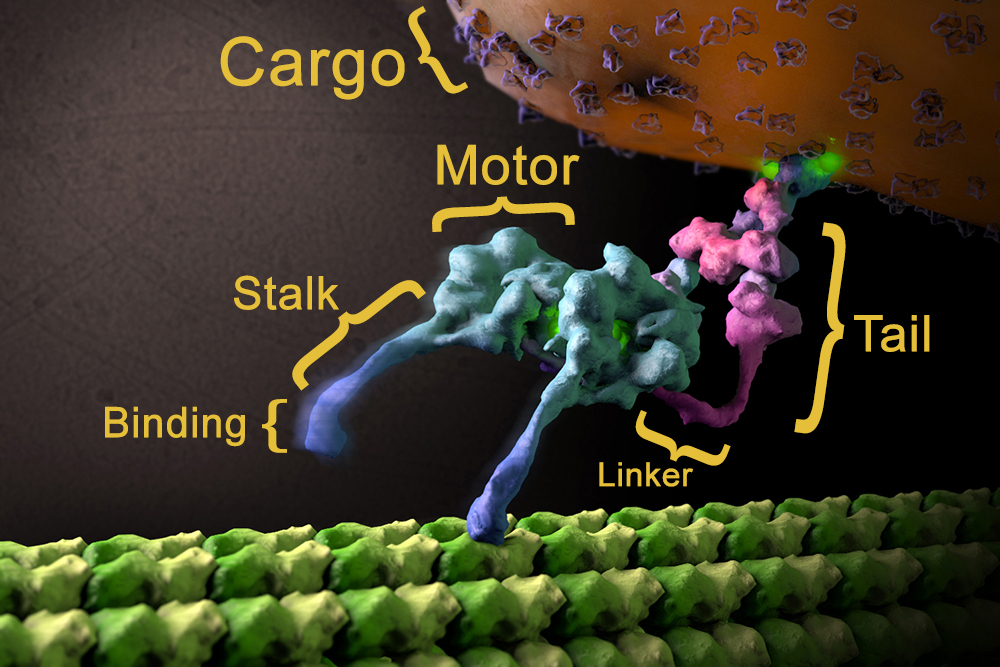
\includegraphics[width=.65\textwidth,keepaspectratio]{../figures/dynein-artist-rendition.jpg}
  \caption{Artist's rendition of dynein bound to a microtubule.}{Two heavy chains (cyan and blue) and several tail proteins (pink) come together to form the dynein motor complex. One monomer's binding domain is bound to the microtubule (green), and the other is diffusing. ATP hydrolysis sites are labeled glowing green. Figure modified. Source: Lander Lab, The Scripps Research Institute \cite{landerartistsrendition}.}
  \label{dynein-artist-rendition}
\end{figure}

Dynein is believed to move by using the energy of ATP to cycle through a sequence of states, each with different spatial relations to the microtubule. By cycling forward through this sequence, the molecule will end up in the same state it began, but moved forward a small amount. This sequence of states is known as the mechanochemical cycle \cite{cianfroccoreview}. The goal of this project is to create a mathematical model of the mechanochemical cycle and verify that it can reproduce experimental dynein stepping data. There are several types of dynein which all behave slightly differently. This project will focus on cytoplasmic dynein-1, hereby referred to as dynein.\\

\subsection{Why do cells need motor transport?}
Cells are organized, heterogenous structures which respond quickly to their environments. This means that cells require a mechanism for rapidly moving components to precise locations within the cell. This can be a challenge, since cells are fairly large compared to the proteins which compose them. A human fibroblast cell has a volume of roughly 2000 $\mu\text{m}^3$\cite{fibroblastvolume}, corresponding to roughly $8 \mu \text{m}$ in diameter. In comparison, human hemoglobin has a diameter of roughly $5 \text{nm}$ (PDB id 5ME2), a $10^3$ factor decrease in size.\\

Diffusion, or random motion of molecules due to collisions with solvent (i.e. Brownian motion), is one possible process cells could use to transport biomolecules. Diffusion has two problems: it is slow and nondirected. The expected distance covered for one-dimensional Brownian motion after time t was found by Einstein to be \cite{einstein-paper}:

\begin{equation}
  \label{diffusion-equation}
  \langle x\rangle = \sqrt{2Dt}
\end{equation}
%
where D is the diffusion constant describing the diffusability of the biomolecule. For a medium-sized (140kD, 1D = weight of H atom) protein with a diffusion constant $D = .2 \mu \text{m}^2/\text{s}$ \cite{diffusionconstants}, it would take about a month to travel across a millimeter-sized cell. In contrast, it would take dynein, which travels at roughly 100nm/s \cite{weihongpaper}, a much more reasonable three hours to do the same. \\%% Figure (\ref{fig:diffusion_vs_dynein}) demonstrates how motor transport quickly outstrips diffusion in a cell.\\

%% \begin{figure}[h]
%%   \centering
%%   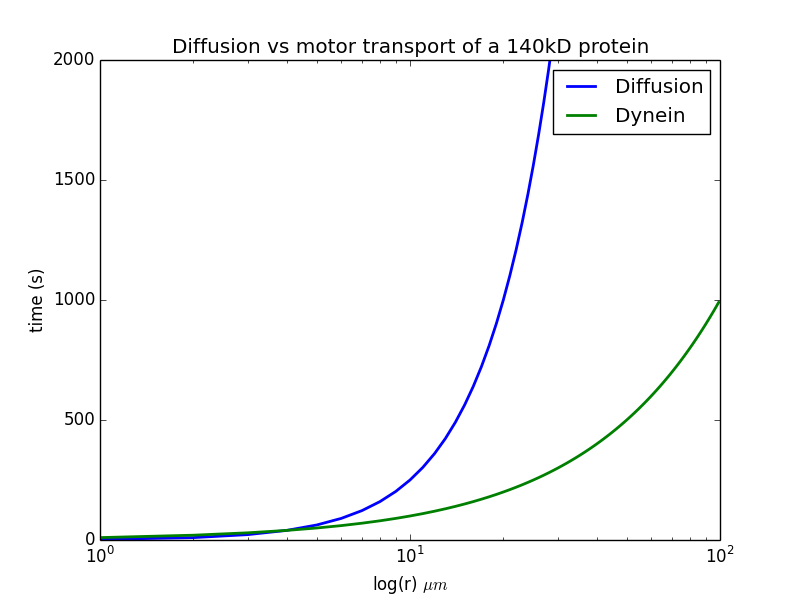
\includegraphics[width=.65\textwidth,keepaspectratio]{../figures/diffusion_vs_dynein.png}
%%   \caption{Passive diffusion vs motor transport rate}{Plot comparing the diffusion rate of a 140kD protein with a diffusion constant $D = .2 \mu m^2/s$ with a dynein motor travelling at 100nm/s.}
%%   \label{fig:diffusion_vs_dynein}
%% \end{figure}

Another advantage of motor transport is that microtubules can be highly specific in their location in the cell. During cell division chromosomes line up at the center of each cell in a plane. Such a geometrically precise shape requires some sort of directed motion which a random process could never provide.\\

\subsection{What role does dynein play in the cell?}
One of dynein's primary jobs is to transport cellular cargos such as organelles, vesicles, mRNA, cytoskeletal filaments and certain proteins from place to place in the cell. Dynein also plays a role in positioning and breaking down the nucleus, cell death, spindle formation and the placement of other important cellular structures \cite{valetoolbox}.\\

Dynein walks along cellular tracks called microtubules (MTs). MTs are long polymers of alternating $\alpha-$ and $\beta-$ tubulin subunits. MTs are polar, meaning they have a distinct directionality based on the orientation of the tubulin proteins which comprise them. One pole, called the minus end, is where they initiate formation, typically at a MTOC (microtubule organizing center) around the center of the cell. The other pole, the plus end, is where they grow and shrink from. Kinesin, another type of motor protein, typically walks towards the plus end of the MT. Dynein is unique in that it walks towards the minus end, making it a minus end-directed motor. This lends it to a particularly important function inside neurons known as retrograde transport.\\

Neurons have cell bodies at their centers and axons which grow outwards. Axons are long, narrow structures extending up to a meter in length in humans. Cell bodies contain nuclei and important organelles for synthesizing proteins, but growth of axon tips is vital for neuron function. This means bidirectional motor transport between axon tips and cell bodies is very important in neurons, since diffusion would not be quick enough. Retrograde transport is transport from the axon tip to the cell body. Cargo includes vesicles full of proteins ready to be broken down in the cell body and microtubule fragments to be returned from the axon tip \cite{neuroanatomy}. Because microtubule minus ends are found in the cell body, dynein's minus end-directed nature makes it the only protein capable of retrograde transport. An interesting question is, if proteins like dynein are synthesized in the cell body but needed at the axon tip to perform retrograde transport, how do dynein get to the tip? The answer is shown in Figure (\ref{retrograde-transport}): kinesin, a plus end-directed motor, takes dynein to the tip from the cell body.\\

\begin{figure}[h]
  \centering
  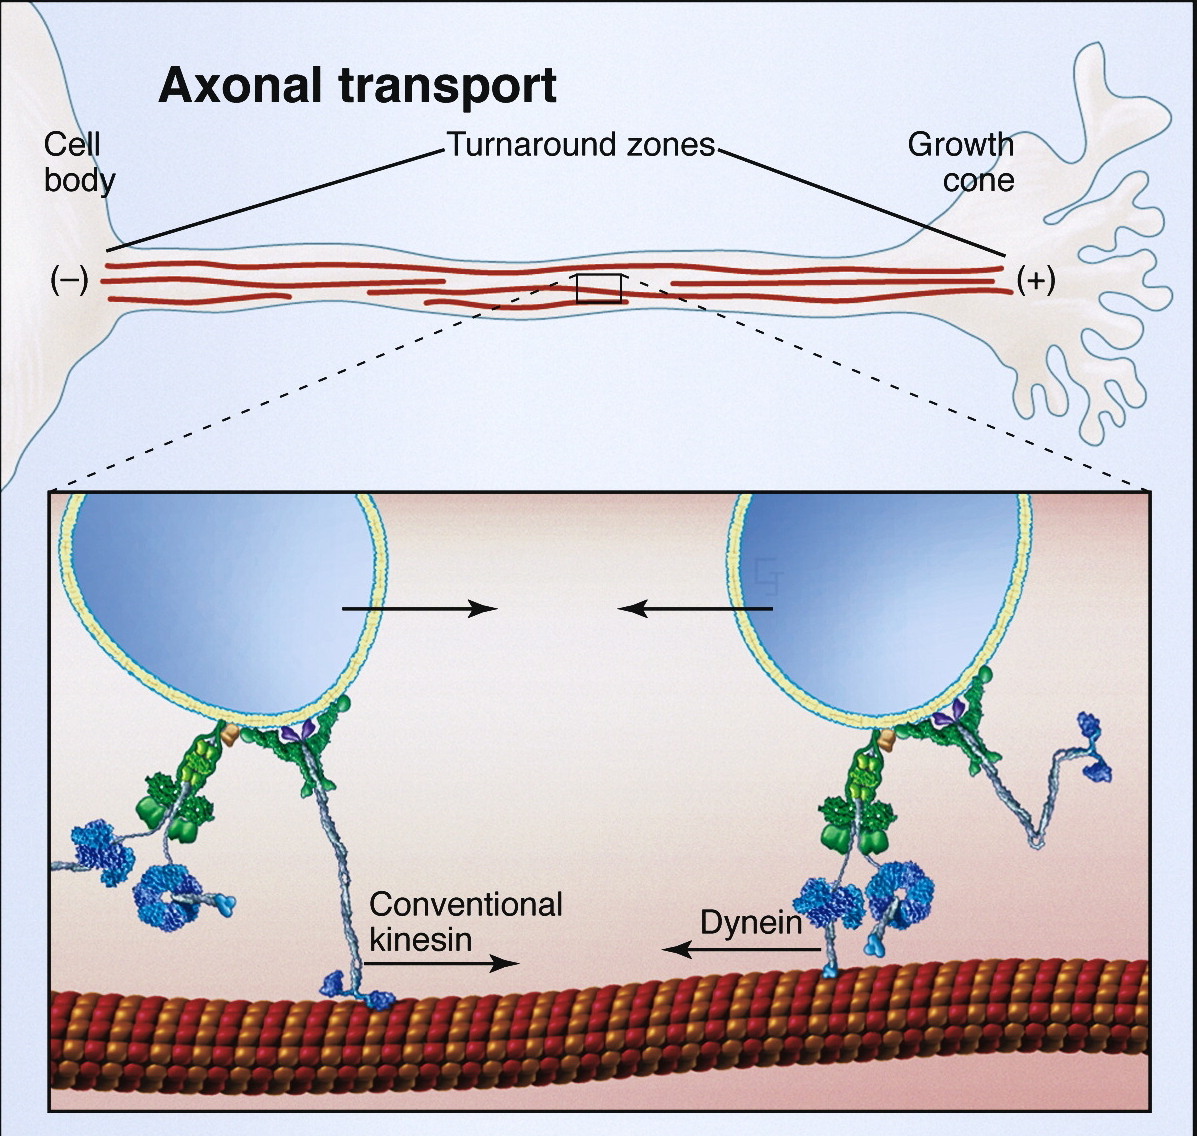
\includegraphics[width=.65\textwidth,keepaspectratio]{../figures/retrograde_transport.jpg}
  \caption{Dynein transport to neuron growth cones.}{Dynein and kinesin collaborate to move cargo between the neuron body and axon tip. The oppositely-directed motors take turns transporting each other, along with cargo for building the axon growth cone. Image from \cite{valetoolbox}.}
  \label{retrograde-transport}
\end{figure}

\subsection{Dynein structure}
As shown in the crystal structure in Figure (\ref{fig:pdb-motm-dynein}), a dynein motor is a fusion of two identical subunits, or monomers, each with binding, stalk, motor and tail subdomains. Each of these subunits has a unique purpose for the motor.\\

Dynein is a fusion of two identical proteins, referred to as monomers. A single monomer, depicted in (\ref{fig:pdb-motm-dynein}), is composed of a microtubule-binding domain (MTBD), a stalk, a buttress, a motor domain, a linker and a tail. The MTBD is responsible for binding to the microtubule. The stalk links the motor domain to the MTBD and carries information about the state of the motor to the MTBD. The motor domain hydrolyses ATP and performs the main conformation changes involved in the step \cite{FRETstatepaper}. The linker connects the tail to the motor and also changes conformation during the step. The tail is a binding site which interacts with several binding partners, including the tail of a twin monomer.\\

\begin{figure}[h]
  \centering
  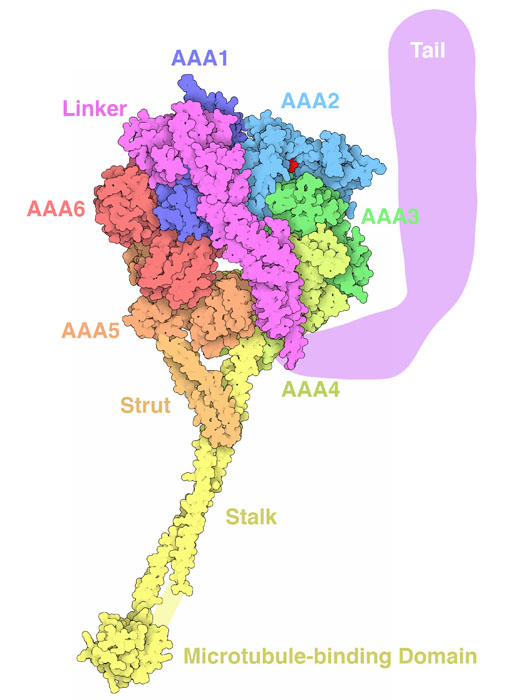
\includegraphics[width=.5\textwidth,keepaspectratio]{../figures/pdb-motm-dynein}
  \caption{Structure of a dynein monomer.}{A cryo-electron microscopy-inspired image detailing the subcomponents of a single dynein monomer. The microtubule-binding domain (MTBD) connects to the motor domain via a coiled coil known as the stalk. The six AAA regions provide structure for the motor domain, and AAA2 conducts the ATP hydrolysis. The linker is a flexible region which connects the motor domain to the tail. One of the main roles of the tail is connecting a monomer to its twin to form the dynein complex. Image from \cite{pdb-motm-dynein}.}
  \label{fig:pdb-motm-dynein}
\end{figure}

\subsection{Why is dynein interesting?}
Selective domain labeling indicates dynein's stepping pattern is highly varied \cite{reck2006single, weihongpaper}. These studies show dynein's stepping pattern to be stochastic and weakly forward-directed. As shown in Figure (\ref{fig:weihong-steps}), dynein takes many backwards steps, and also many steps with components perpendicular to the microtubule. This indicates the process dynein uses to generate motion has a stochastic component to it. In contrast, kinesin is known to take very regular 8nm steps in the absence of large forces \cite{kinesin-step-size}. For reference, the diameter of a microtubule is roughly 25nm.\\

\begin{figure}[h!]
  \centering
  \includegraphics[width=0.49\textwidth]{../figures/weihong-step-size}
  \includegraphics[width=0.49\textwidth]{../figures/weihong-off-axis-steps}
    \caption{Experimental dynein stepping behavior histograms.}{Left: Size of steps taken by dynein motor parallel to microtubule. Positive axis corresponds to steps towards the microtubule minus-end. Right: Size of ``off-axis'' steps taken by the dynein motor perpendicular to the microtubule. Figure modified from \cite{weihongpaper}.}
  \label{fig:weihong-steps}
\end{figure}

Kinesin and dynein, although of very different evolutionary origin \cite{hook-family}, have very similar stepping cycles. Both proteins bind bipedally to microtubules. Both proteins use ATP hydrolysis to leverage against a linker domain, pushing the motor domain forward. Both proteins couple their nucleotide and MT-binding states \cite{vale-kinesin-cycle}. How, given the large number of similarities between these motors, does dynein achieve such a radically different stepping pattern than kinesin? Elucidating how the structural differences between the motors give rise to the differences in dynamics would provide lots of important information on how the machines fine-tune their stepping.\\

A major factor which could contribute to differences in stepping is each protein's size. Kinesin proteins are generally 100-200 kD in mass, whereas dynein is on the order of 1mD. As shown in Figure (\ref{fig:kinesin-vs-dynein}), the dynein motor domain is much bigger than the kinesin motor domain. Another key difference is the separation between ATP hydrolysis sites on either protein. Kinesin's ATP hydrolysis site is inside the globular microtubule-binding domain. In contrast, Dynein binds to the MT with its MTBD, colored yellow in Figure (\ref{fig:kinesin-vs-dynein}), and hydrolyses ATP in its motor domain, which is colored cyan. This distance is close to 20nm in length - much longer than kinesin. This large separation might act like a loose ``leash,'' allowing the binding domain to diffuse freely around the microtubule. Kinesin has a much more rigid leash, as shown in the bottom pane of (\ref{fig:kinesin-vs-dynein}). This more rigid leash may prevent diffusion from happening as much.\\

\begin{figure}[H]
  \centering
  \begin{minipage}{0.3\textwidth}
    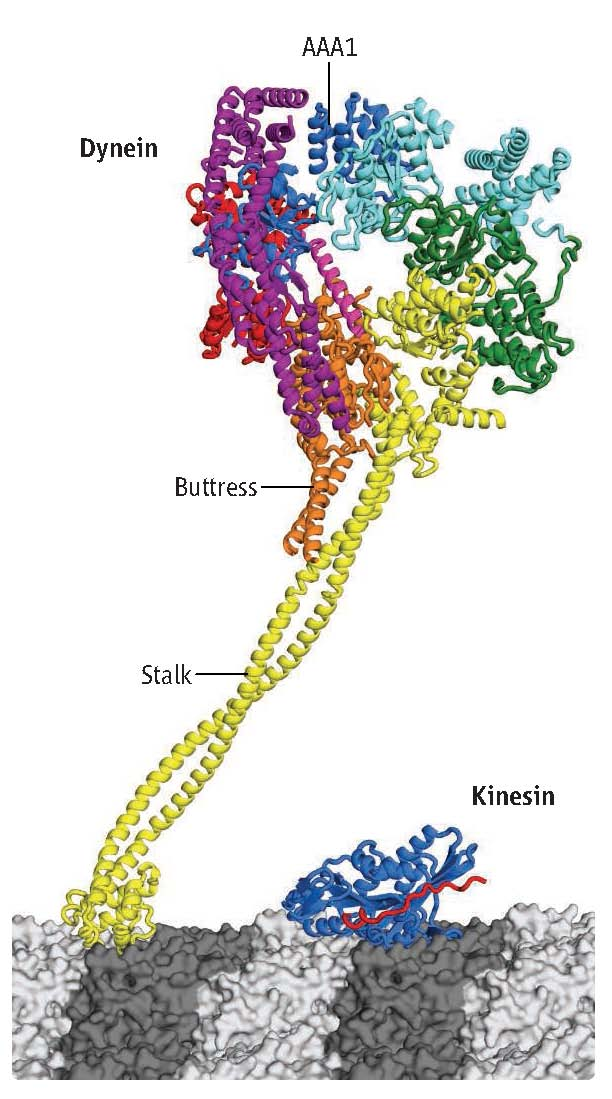
\includegraphics[width=\textwidth,keepaspectratio]{../figures/kinesin_vs_dynein}
  \end{minipage}
  \begin{minipage}{0.65\textwidth}
    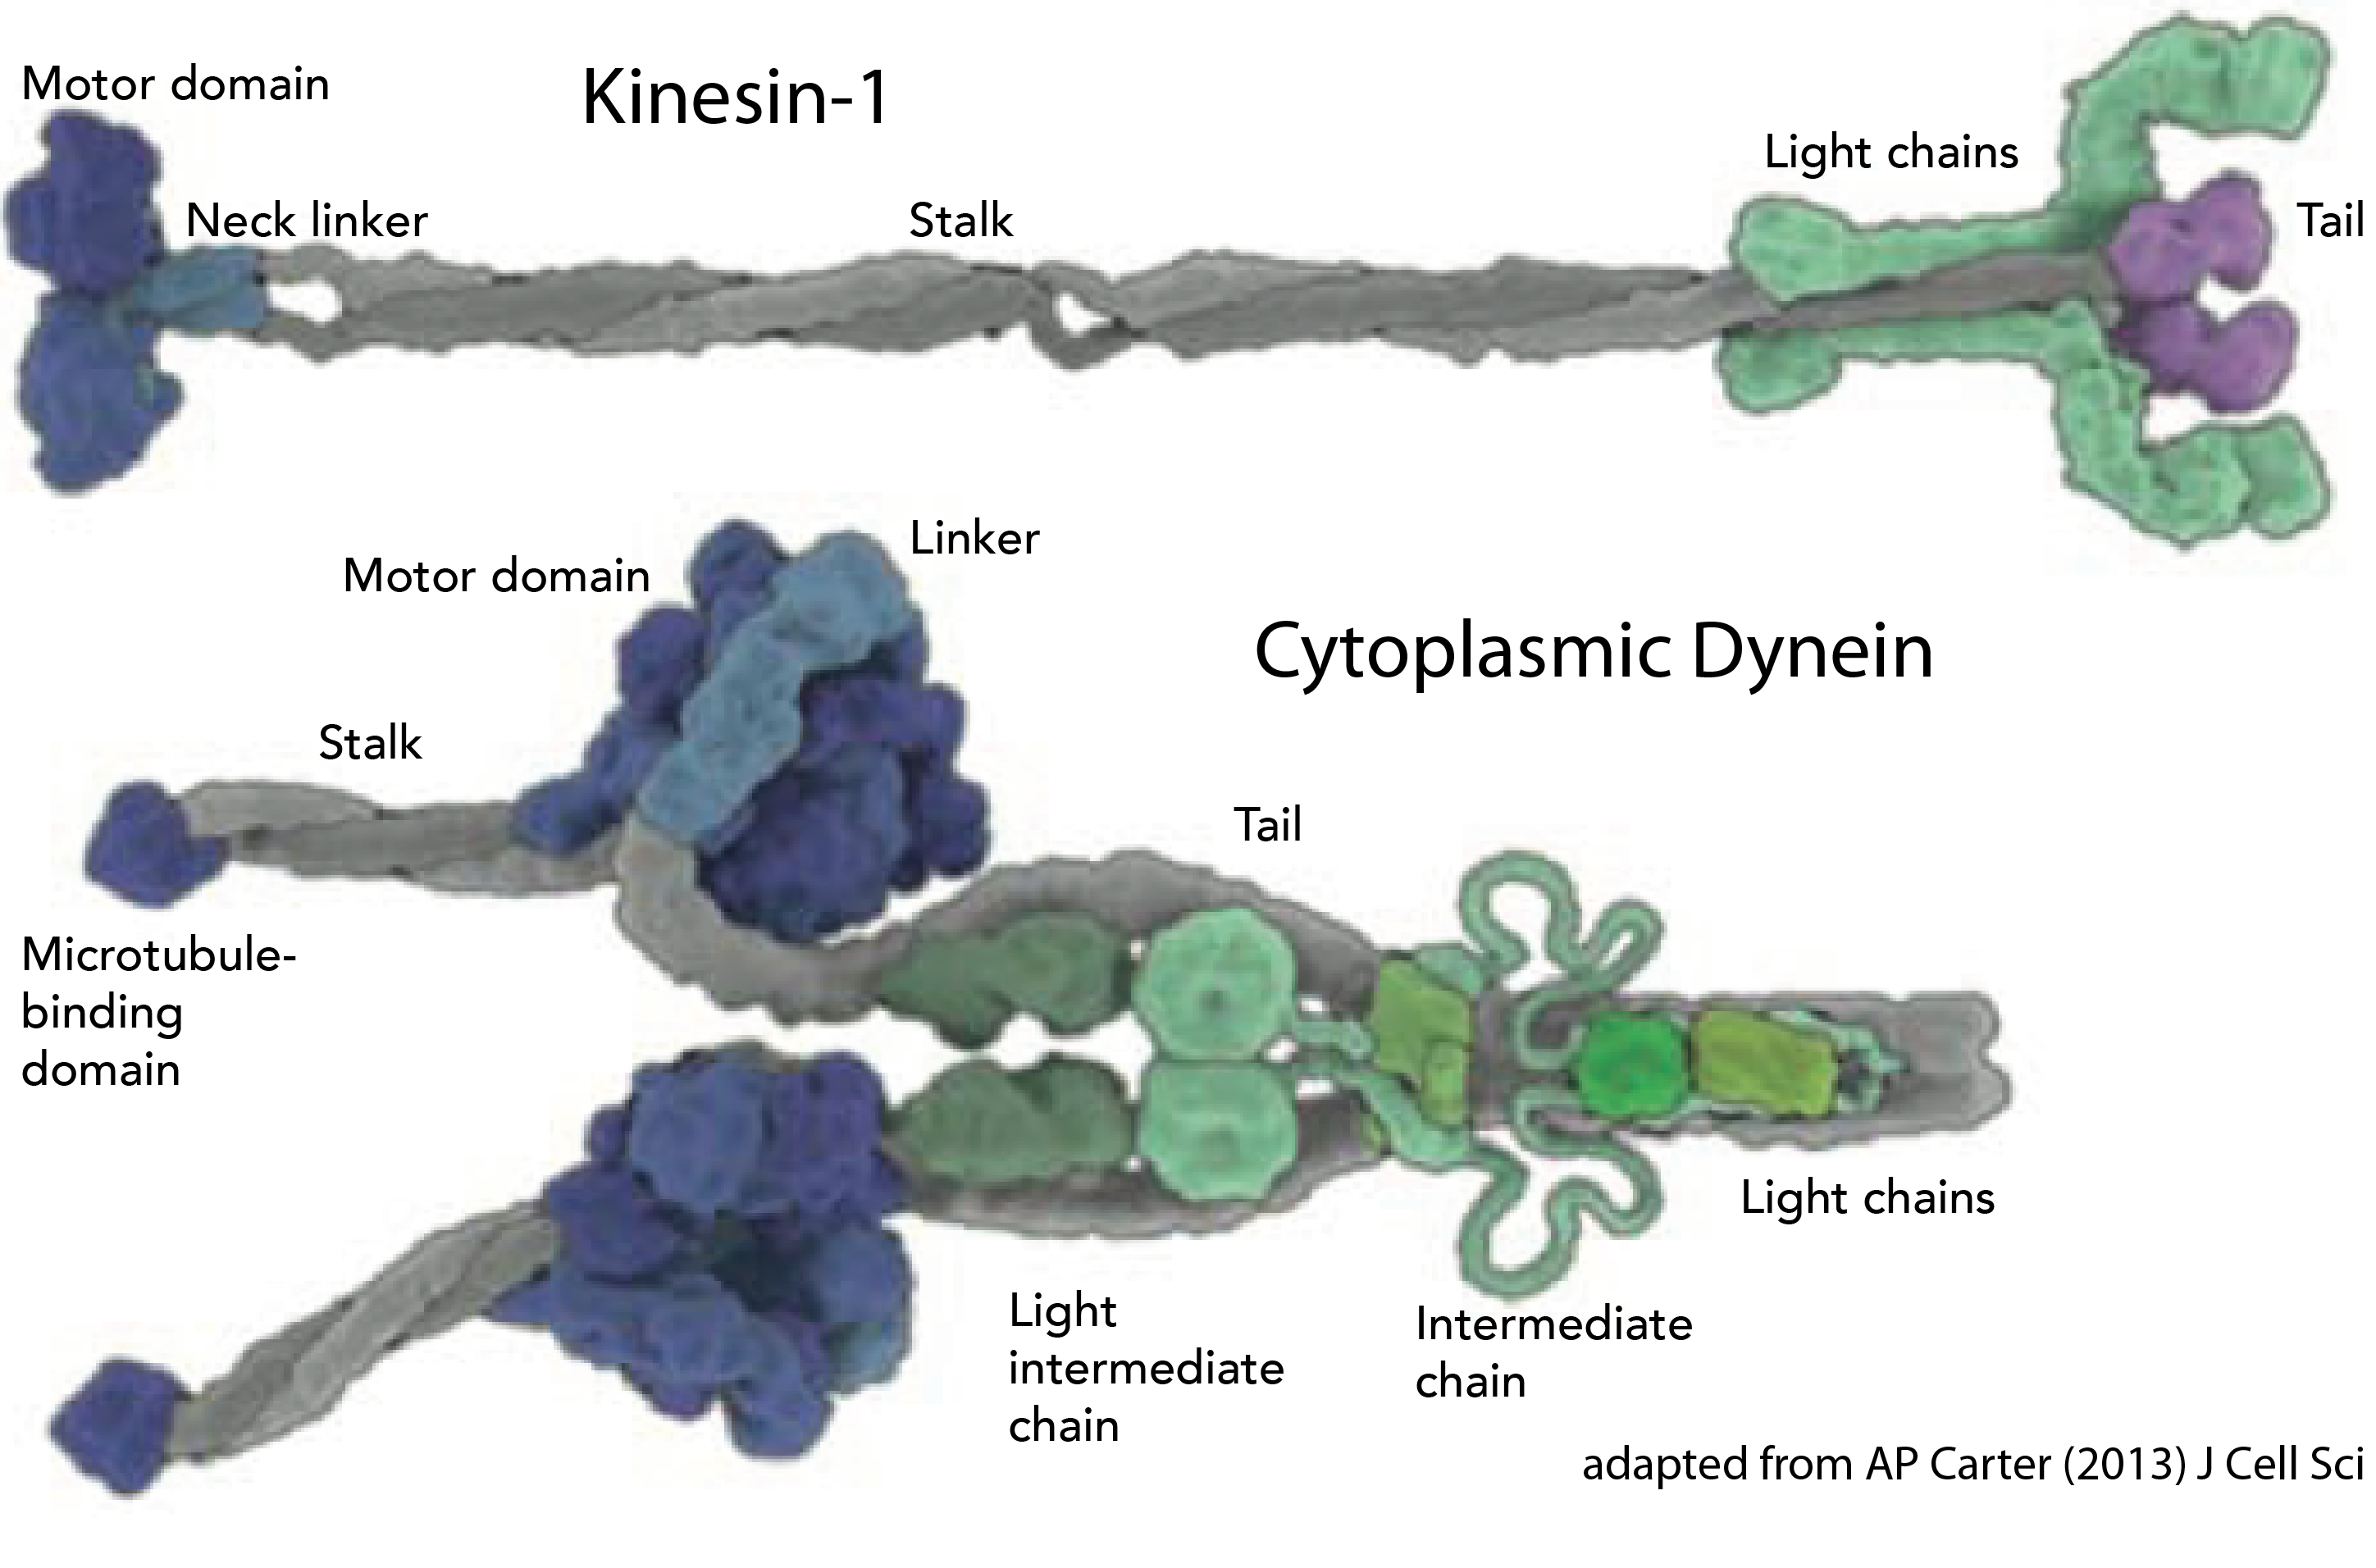
\includegraphics[width=\textwidth,keepaspectratio]{../figures/kinesin_vs_dynein_2}
  \end{minipage}
  \caption{Structural comparison of dynein and kinesin}{Left: Comparison of crystal structures of the motor domains of dynein and kinesin bound to a microtubule. Image from \cite{kinesin-vs-dynein}. Right: Full motor complexes of dynein and kinesin inspired by cryo-EM microscopy. The blue regions on the right image of either protein are the motor domains, which are pictured in the left crystal structures. Not present in the left cyrstal structures are the tail and intermediate chains of either protein. Right image from \cite{kinesin-vs-dynein-2}.}
  \label{fig:kinesin-vs-dynein}
\end{figure}

\section{Dynein Stepping Background}
Biophysicists and molecular biologists have conducted experiments over the past twenty years which shed light on how the dynein motor might walk. The full mechanism is not known, but several known behaviors of dynein can be taken together to construct a model for how the motor walks.\\

\subsection{ATP cycle influences conformational state}
Dynein is known to occupy multiple discrete conformational states depending on its environment. In particular, the concentration of ATP and microtubules is known to alter the shape dynein takes on. A FRET (fluorescence resonance energy transfer) study attached fluorophores to dynein's motor and tail and measured the average distance between the two \cite{FRETstatepaper}. It was found that average distance increased or decreased depending on the nucleotide bound to dynein, indicating the motor takes on different conformations for different bound nucleotides. Dynein unbound to nucleotide, or frozen in ATP or ADP-bound states, had a similar tail-motor distance. However, when the motor was stuck in an ADP-Pi state, with ATP hydrolyzed but phosphate not yet released, the tail-motor distance was increased. This suggests that dynein starts its cycle with no nucleotide, binds ATP, hydrolyzes ATP, enters the ADP-Pi state and changes conformation to a far tail-motor distance, then releases phosphate, moves back to its original close tail-motor conformation, then ejects ADP and starts over.\\

Studies suggest that near/far tail-motor conformation changes are not due to lengthening of the stem linking the two domains, but rather a change in position of the head relative to the tail \cite{FRETstatepaper, burgess-paper}. Cryo-electron microscopy images of the dynein motor shown in Figure (\ref{fig:cryo-em-angles}) demonstrate the differences in conformation in the nucleotide-free and ADP-Pi state. The shifting of the linker domain in the ADP state is known as the powerstroke, and is believed to be the principle cause for dynein's forward step.\\

\begin{figure}[h]
  \centering
  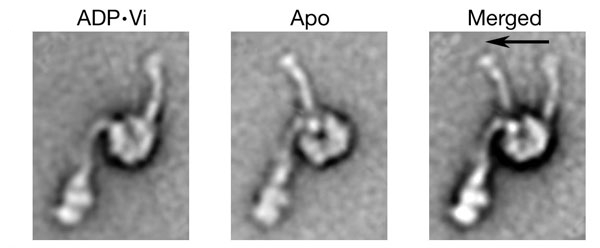
\includegraphics[width=.65\textwidth,keepaspectratio]{../figures/burgess-dynein-angles}\\
  \hspace{1cm}
  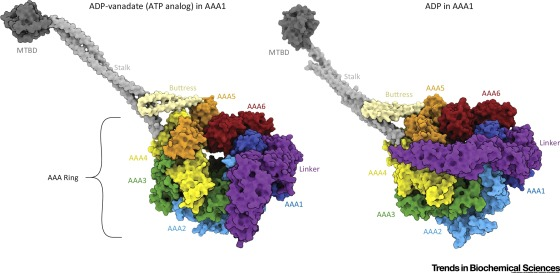
\includegraphics[width=.95\textwidth,keepaspectratio]{../figures/linker-swing}
  \caption{Dynein conformation change during a step.}{Top: Cryo-electron microscopy images of axonemal dynein in two different nucleotide states. Top left: dynein frozen in ADP-Pi state. Top middle: dynein without nucleotide. Top right: two states superimposed on one another. Figures from \cite{burgess-paper}. Bottom: X-ray diffraction-inspired image of a motor in two nucleotide states. Bottom left: motor in ADP-Pi state. Bottom right: Motor in ADP state. The linker undergoes an approximately 40 degree swing between these two states known as the powerstroke. Figure from \cite{bhabha-paper}.}
  \label{fig:cryo-em-angles}
\end{figure}

Crystal structures of cytoplasmic dynein-2, a relative of dynein, indicate that ATP-Pi binding to the motor domain induces a conformation change in the motor domain, which alters the angle at which the motor binds to the tail \cite{carter-paper}. Taken together, these results indicate that as the motor binds and hydrolyzes ATP, it undergoes a conformation change which physically moves the motor relative to the tail.\\

%% \textbf{TODO: look at \cite{nicastro} and \cite{schmidt-carter} to see if they can add to this discussion}

\subsection{Microtubule and nucleotide states are coupled}
Dynein is known to bind to the microtubule at a location known as the $\alpha$-$\beta$ polymerization site \cite{redwineMTBDcomplex}. This site occurs roughly every 8nm, indicating dynein is restricted to forward step sizes which are multiples of 8nm. The motor is also capable of stepping sideways \cite{weihongpaper}, indicating total displacements which are not multiples of 8nm.\\

The nucleotide state of the motor is not the only determiner of dynein conformation; microtubule binding state has also been shown to influence conformation. A study on the MTBD-MT complex indicates the stalk connecting the motor and MTBD can take on two major conformations, depending on whether the MTBD is bound to the MT or not \cite{mt-atp-coupling}. The conformation of the stalk has been shown to communicate information between the motor and MTBD. In the presence of microtubules, the ATPase rate of the motor is increased 25-fold. This indicates the stalk communicates MT-binding state of the MTBD to the motor, increasing its ATP hydrolysis rate. The communication happens the other way, as well. Treating dynein with ATP causes MT-binding rate to drop 15-fold, indicating ATP-binding at the motor decreases MT-binding rate at the MTBD.\\

In addition to a bidirectional linking between ATPase rate and MT-binding, stalk state has been shown to directly influence motor conformation \cite{mt-atp-coupling}. When the stalk is allowed to freely transition between bound and unbound states, the motor can also transition between near and far tail/motor states. However, when the stalk is frozen in a particular conformation, the motor loses its transitioning ability. This suggests that the conformations of the two systems are tightly linked.\\

\section{Cianfrocco model for dynein stepping}
\label{sec:cianfrocco-model}
Data presented in the previous sections paints a picture of dynein as a collection of interconnected parts, each cycling through its own collection of states and influencing other parts. Somehow the protein interacts with nucleotides and microtubules in a way that allows it to reliably move through the cell. The Cianfrocco model presented below takes these facts and string them together into cohesive cycles which might explain how dynein walks.\\

Cianfrocco \textit{et. al} \cite{cianfroccoreview} propose dynein achieves motion via transitioning through the cycle of states shown in Fig. (\ref{mech-cycle}). The model claims the primary events in the dynein step are as follows. First, starting with both binding domains attached to the MT, ATP binds to the motor domain, which causes it to change conformation. ATP hydrolysis to ADP-Pi causes further conformation changes. These changes cause the binding domain to release the microtubule, meaning only one binding domain is MT-bound. The free binding domain then undergoes another conformation change known as the ``priming stroke,'' which changes the orientation of the binding domain with respect to the MT. Finally the binding domain rebinds to the MT, causing a final conformation change in the motor which returns it to the beginning of the cycle. The exact order of these events is not precisely known.\\

\begin{figure}[h!]
  \centering
  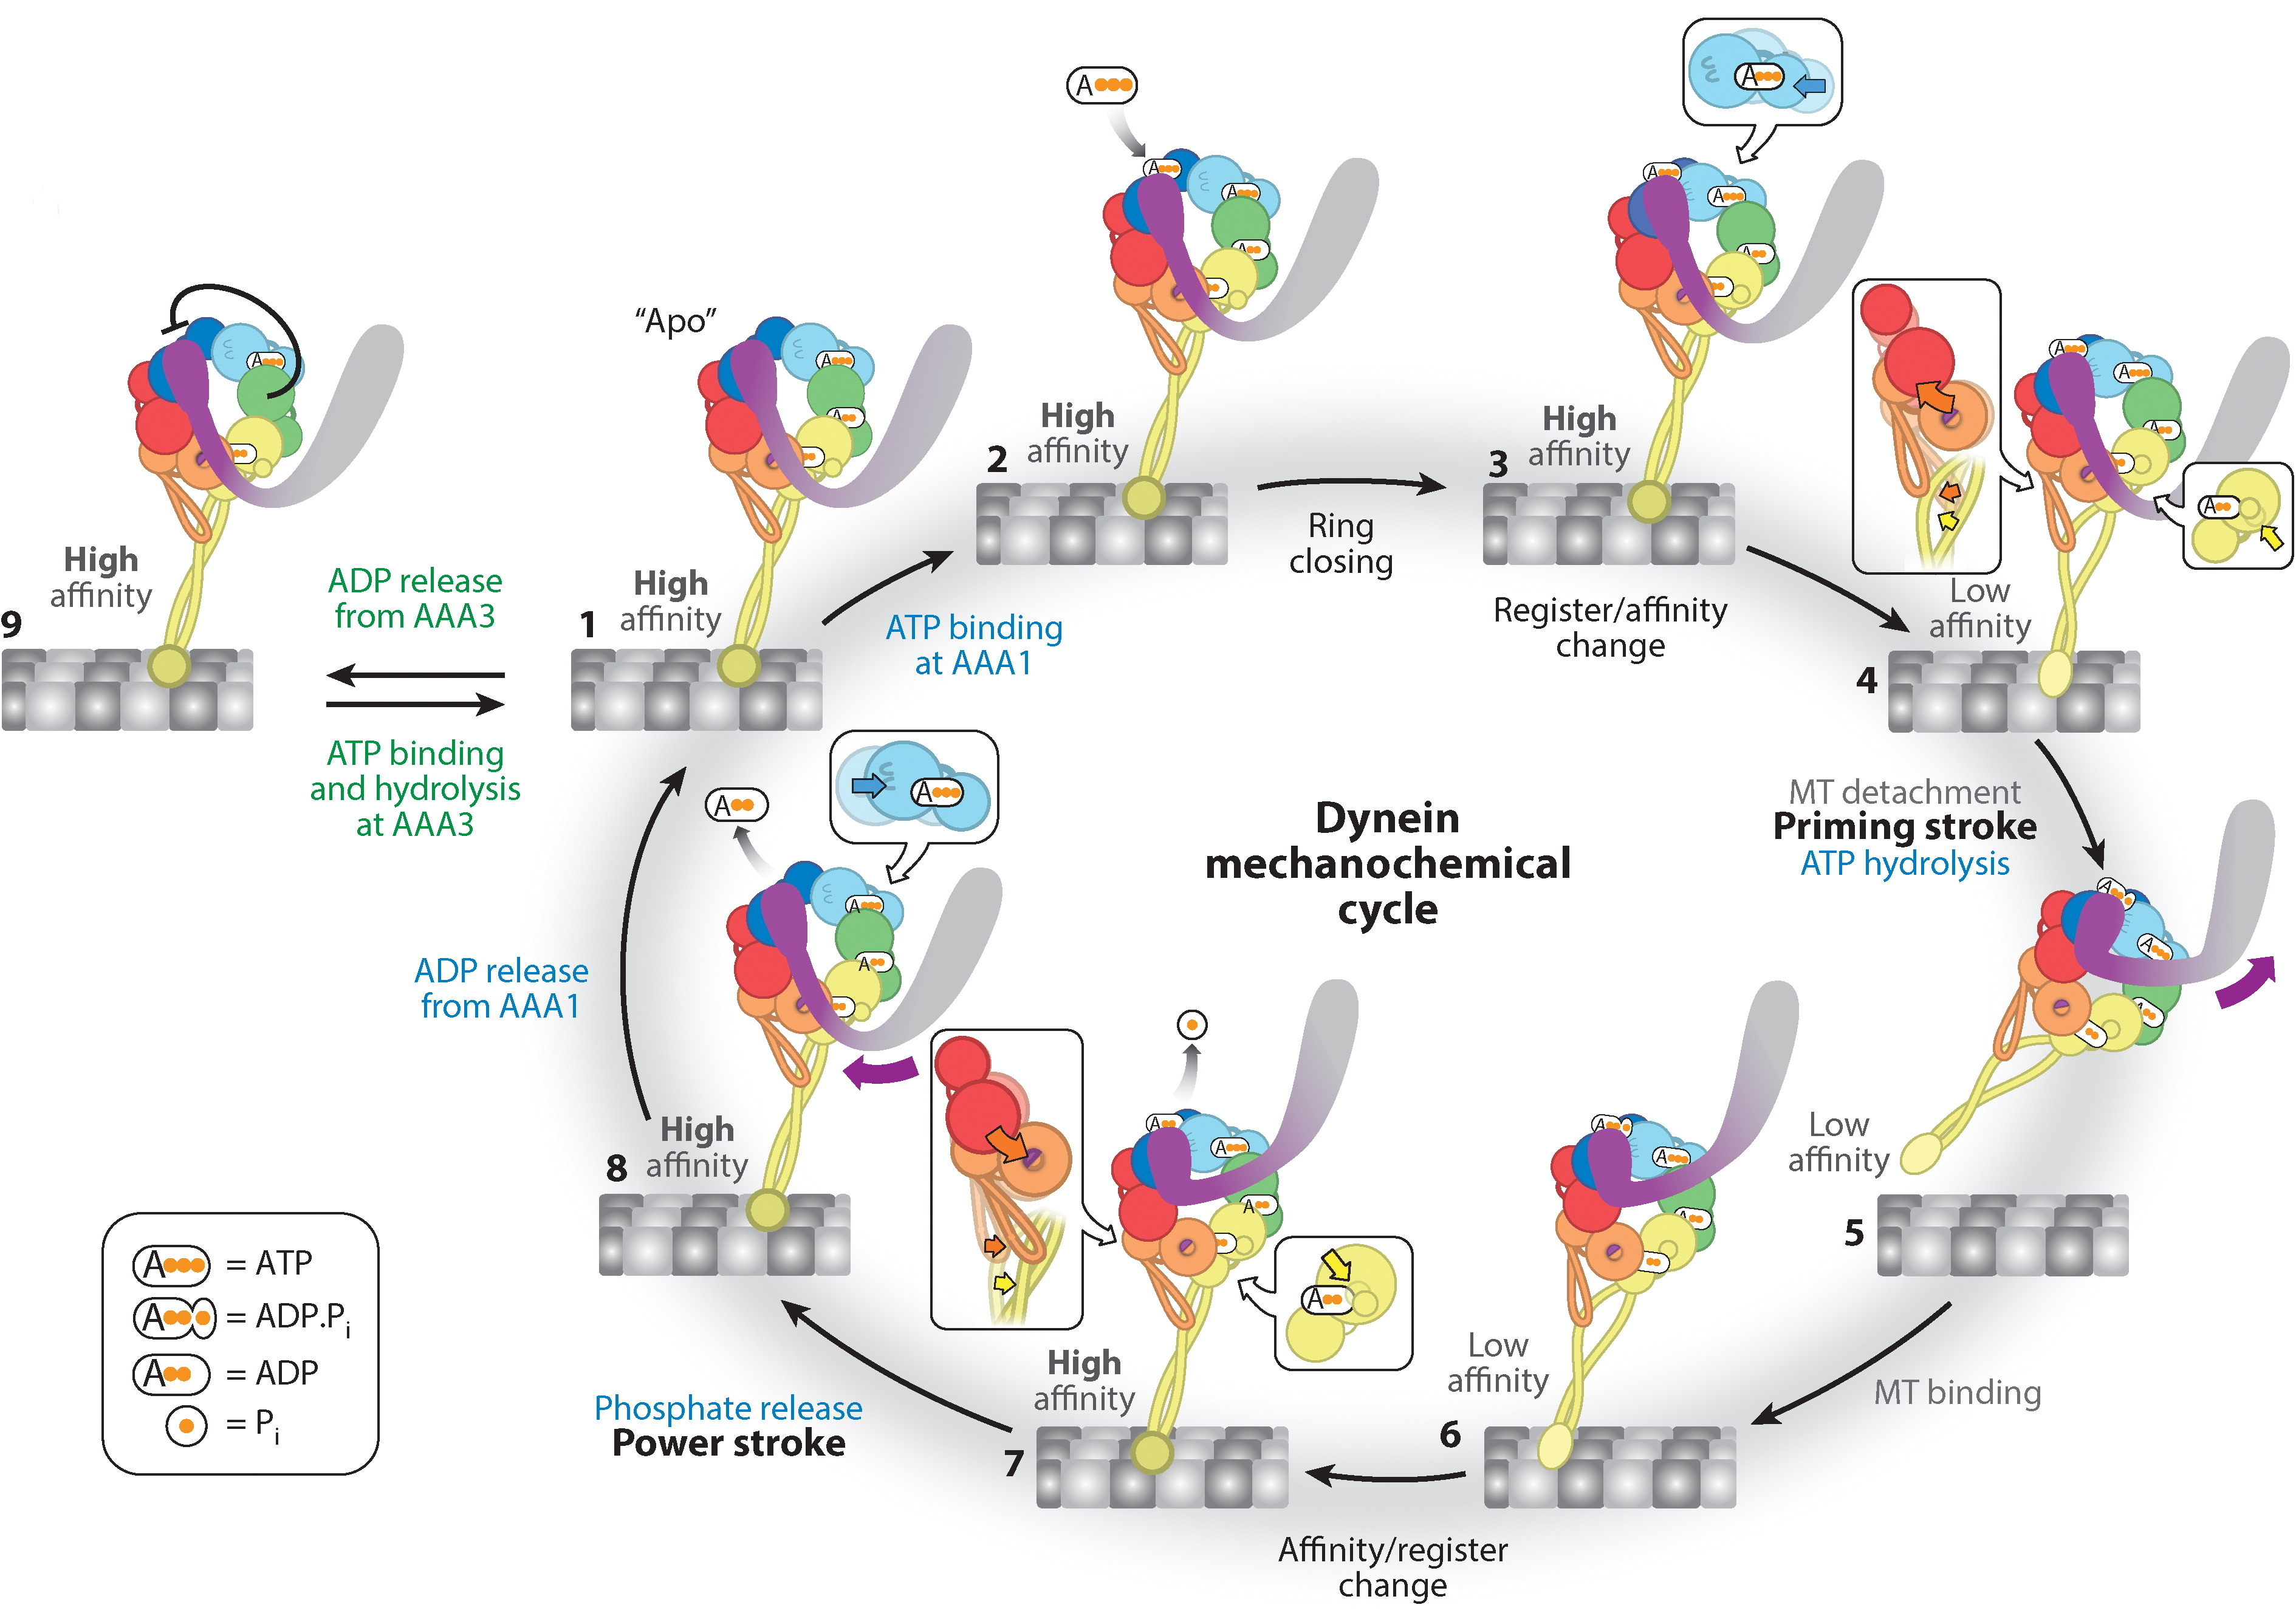
\includegraphics[width=.90\textwidth,keepaspectratio]{../figures/mechanochemical-cycle.jpeg}
  \newcommand\bothbound{\textcolor{blue}{BOTHBOUND}}
  \newcommand\onebound{\textcolor{red}{ONEBOUND}}
  \newcommand\transition{\textcolor{green}{transition?}}
  %% \begin{tabular}{rll}
  %%   \bothbound &
  %%   1 & \begin{minipage}{5in}
  %%     Bound to microtubule and waiting for ATP to arrive.  The
  %%     conformation is ``post-powerstroke''.
  %%   \end{minipage}\vspace{0.5em}\\
  %%   \bothbound &
  %%   2 & \begin{minipage}{5in}
  %%     ATP has bound to the motor at AAA1, but nothing else has changed.
  %%   \end{minipage}\vspace{0.5em}\\
  %%   \transition &
  %%   3 & \begin{minipage}{5in}
  %%     ``The ring has closed'' in the motor, whatever that means.
  %%   \end{minipage}\vspace{0.5em}\\
  %%   \bothbound &
  %%   4 & \begin{minipage}{5in}
  %%     The affinity to the microtubule is dropped, so it is likely to pop off soon.
  %%   \end{minipage}\vspace{0.5em}\\
  %%   \onebound &
  %%   5 & \begin{minipage}{5in} It has popped off of the microtubule!
  %%     Onebound! The equilibrium angle is also changed.  The ATP has
  %%     been hydrolized, but the phosphate is still bound to the motor.
  %%     ``Priming stroke?''
  %%   \end{minipage}\vspace{0.5em}\\
  %%   \onebound &
  %%   6 & \begin{minipage}{5in} It is now bound to the microtubule, but
  %%     with low affinity, and without any loss of phosphate. Question:
  %%     does this happen many times? If so it may still be onebound.
  %%     Otherwise it is probably bothbound.
  %%   \end{minipage}\vspace{0.5em}\\
  %%   \bothbound &
  %%   7 & \begin{minipage}{5in}
  %%     Now it is seriously bound to the microtubule, and the motor
  %%     domain has changed conformation.  This is now ``high affinity.''
  %%   \end{minipage}\vspace{0.5em}\\
  %%   \bothbound &
  %%   8 & \begin{minipage}{5in}
  %%     Phosphate has been released, and our equilibrium angles have
  %%     been changed.  This is the ``power stroke.''
  %%   \end{minipage}\vspace{0.5em}\\
  %%   \bothbound &
  %%   1 & \begin{minipage}{5in}
  %%     The ADP has been released from the motor domain, so it can now
  %%     bind ATP.  Still ``high affinity,'' and still in the
  %%     ``power-stroke'' conformation.
  %%   \end{minipage}\vspace{0.5em}\\
  %%   \bothbound &
  %%   9 & \begin{minipage}{5in}
  %%     While stuck in this ``normal bound'' state, another site on the
  %%     motor AAA3 can lose its ADP, which leaves the motor in a state
  %%     where it cannot directly move on to step 2 (until after
  %%     reversing this).  Controversial?
  %%   \end{minipage}
  %% \end{tabular}
  \caption{Cianfrocco mechanochemical cycle.}{Cycle of states the dynein motor goes through during motion in the Cianfrocco model \cite{cianfroccoreview}.}
  \label{mech-cycle}
\end{figure}

%% \subsection{Other models}
%% Find other models and put them here

%% \section{Brownian dynamics}
%% New section which describes how BD works.

\section{Testing the Cianfrocco model}
One of the main goals of studying dynein is establishing how the motor walks. This can be a difficult task, since direct observation of the protein walking is not currently experimentally possible. Given the experimental challenges, a computational approach seems promising. This approach involves forming a hypothesis on how the motor walks, creating a model which behaves according to this hypothesis, simulating that model, and comparing the simulation's behavior to experimental data. This process can be an efficient way to support hypotheses and guide future research.\\

\subsection{Computational approach}
This project seeks to create a dynamic model of dynein and use it to answer questions. The Cianfrocco model provides a rough framework for the events that go on during the dynein mechanochemical cycle. By augmenting this model with information about dynein's structure and conformation changes occuring during the cycle, a new dynamic model which takes into account both temporal and spatial information can be constructed. This dynamic model can then be simulated under cellular conditions to test how it behaves. Such a model would be ideal, since it would make very precise predictions about how real dynein walks. This simulation would act as an experiment testing the validity of the Cianfrocco model.\\

\subsection{Questions to answer}
The biggest question such a simulation would answer is: does the Cianfrocco model, when applied to a dynein-sized motor with elastic hinges, produce dynein-like stepping? High similarity between simulation behavior and experimental dynein behavior would be a strong positive result supporting the Cianfrocco model. If confirmed to be dynein-like, the simulation could then be used to answer many other questions.\\

Dynein has both angular and linear elasticity between its domains. Angular elasticity, or the flexibility of protein domains relative to each other, may play a large role in dynein's stepping. It is possible that dynein requires its foot domain to diffuse to a high-energy conformation in order to take a step. It is postulated by \textit{Burgess et. al.} \cite{burgess-paper} that changes in angular elasticity may be important for dynein's ability to step at key points in the mechanochemical cycle. Alternatively, it is possible that elasticity is not required, and the angular changes caused by the powerstroke are enough for stepping. By varying the angular elasticity of the model, this simulation could determine the importance of angular elasticity for dynein's step.\\

Another question this simulation could answer is how dynein localizes to its binding site. Microtubules are regular tubulin polymers with MTBD binding sites roughly every 8nm. Dynein can take steps at integer multiples of this length, but the 8nm step is its most favored. Why is this? Does the MTBD drag along the microtubule until it hits a binding site? Or, does it diffuse high above the microtubule, randomly descending until it finds a place to bind. This simulation could answer that question by outputting MTBD positions over time.\\

Why does dynein step differently than kinesin? Kinesin follows a similar mechanochemical cycle to dynein. By modifying the stepping cycle, shrinking inter-domain distance and changing conformation angles of the dynein model, it may be possible to create a rough kinesin dynamic model. This model could then be tested for similarity to experimental kinesin. If kinesin behavior was replicable, then comparisons between the models could be readily made. Does kinesin step like dynein when its size is increased? Does dynein step like kinesin when its conformation angles are made rigid? By varying the spatial representation of the two models, it might be possible to determine why the two motors step differently.\\

Kinesin and dynein generally travel in opposite directions along the microtubule. Why is this? Both proteins bind to the same place on the microtubule \cite{kinesin-dynein-mt-overlap}, so the binding site can't determine directionality. It is possible that not the binding site, but the angle at which the protein binds to the microtubule is what determines its stepping direction. If it turns out that kinesin can be successfully modelled using the same dynamic model, then this question could possibly be answered. If altering the microtubule binding angles of dynein and kinesin reverses their directionality, it may be that binding angle is all it takes to determine motor directionality.\\

%% \textbf{Things which are known about dynein which support the Cianfrocco model}
%% \begin{itemize}
%% \item AAA1 only ATPase necessary for motility, which is why we don't include the other ATPases in our model \cite{cianfroccoreview}
%% \item AAA5 mediates stalk register changes Schmidt H, Zalyte R, Urnavicius L, Carter AP. 2014. Structure of human cytoplasmic dynein-2 primed for
%%   its power stroke. Nature 518:435–38
%% \item Linker moves as response to AAA1 nucleotide binding Burgess SA, Walker ML, Sakakibara H, Knight PJ, Oiwa K. 2003. Dynein structure and power stroke. Nature
%%   421:715–8
%% \item Crystal structures with Vanadium-Adp show dynein in the pre-powerstroke state, hinting that ADP-Pi-bound dynein takes on a different conformation than ADP-Pi free dynein
%% \end{itemize}

\newpage
\chapter{Theory}
\label{chap:Theory}

\section{Model overview}
The model constructed in this thesis is meant to approximate how a protein with dynein's structure which underwent the conformational changes described in the Cianfrocco model (\ref{sec:cianfrocco-model}) would behave in a cell. In order to be compared to experiment, the model should output spatial information about dynein's rough conformation at all times during the simulation. Creating such a model is a balance between accuracy and computational efficiency. The model must be complex enough to correspond well to dynein, but not be so complex that it cannot be simulated in a reasonable amount of time. Molecular dynamics, a technique which simulates the individual amino acids in a protein, would be highly accurate, but would be prohibitively expensive to simulate a dynein step. Thus, many approximations are made about dynein to simplify the simulation.\\

\begin{figure}[h]
  \centering
  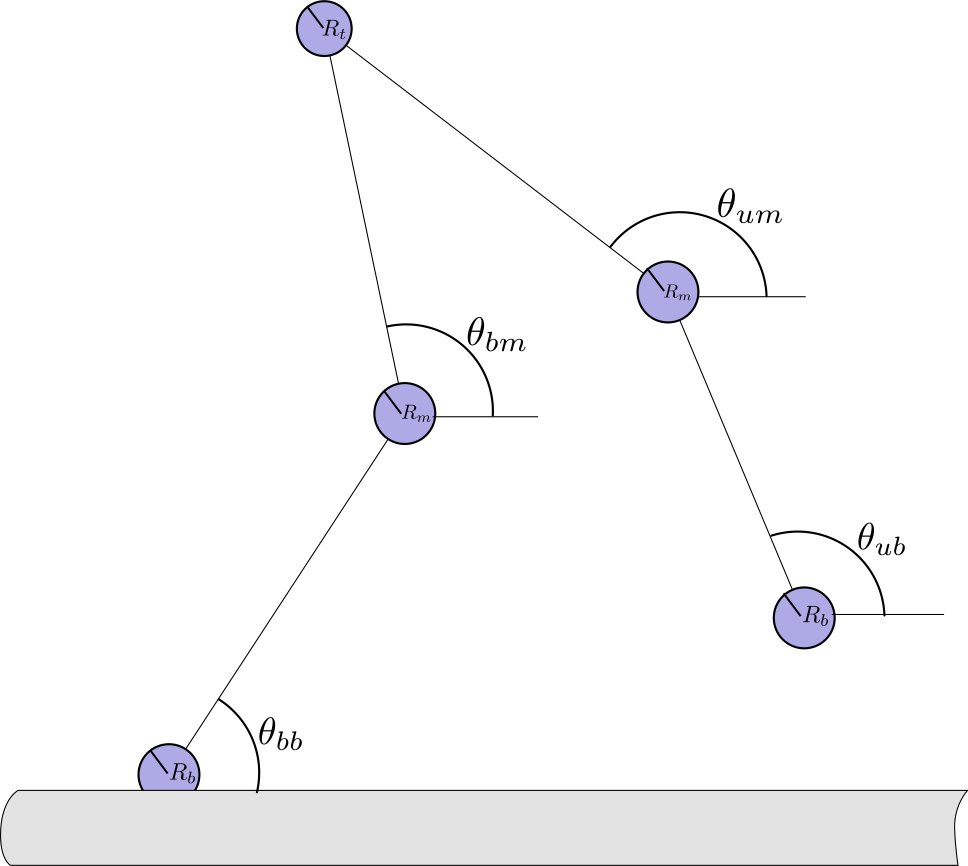
\includegraphics[width=.45\textwidth]{../figures/theory-onebound}
  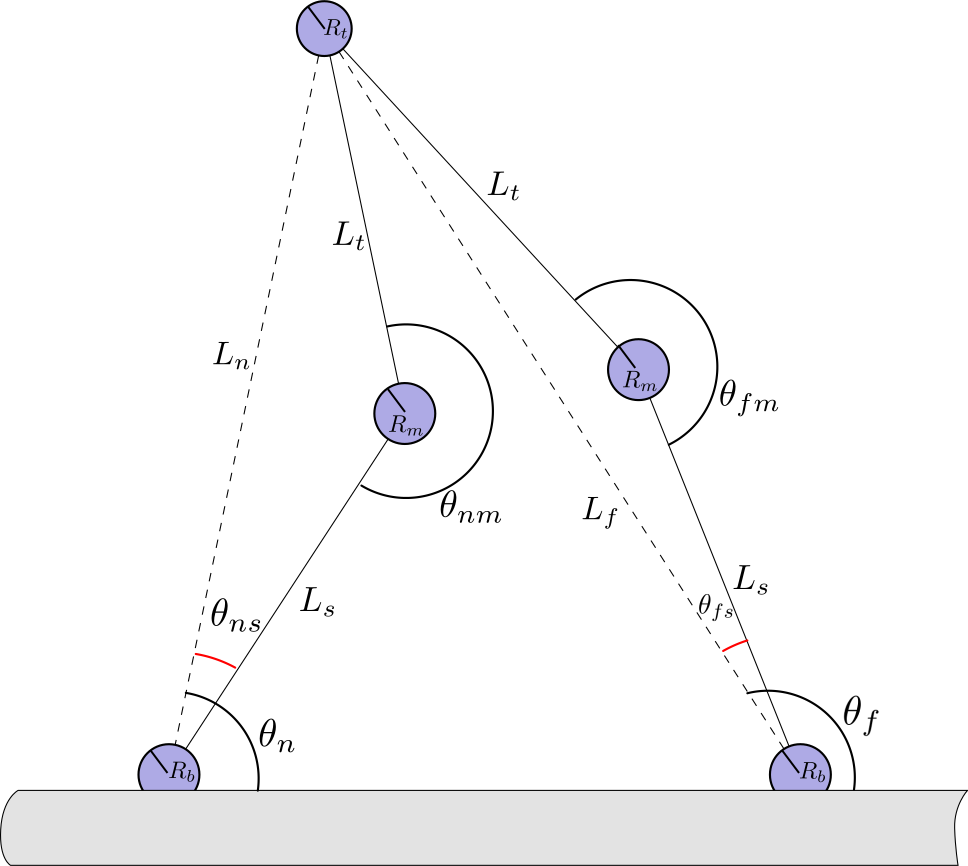
\includegraphics[width=.45\textwidth]{../figures/theory-bothbound}
  \caption{Spatial representation of the dynein dynamic model.}{Dynein is simplified to two two-dimensional point-particle systems. The left ``onebound'' system represents dynein when one MTBD is unbound, and the right ``bothbound'' system represents dynein with both MTBDs bound. Five points in total represent the two MTBDs, two motor domains and one tail domain. Each model's orientation is defined by a set of angles, four in the onebound case and two in the bothbound case. These points are connected by rigid rods. Although approximated as points, each domain has a radius $R$ associated with it used for drag calculations.}
  \label{fig:theory-intro}
\end{figure}

\subsection{Summary}
The model is composed of two separate systems of five point particles, with each point representing a domain of dynein: two binding domains, two motor domains and one tail domain. Physical representations of these two systems are shown in Figure (\ref{fig:theory-intro}). The points are connected together by rigid rods, and the sytems are defined by the angles the rods make at each point. These angles are free to swivel. Each point thus acts somewhat like a ``hinge'' which can open or close. These two systems represent different modes dynein can be in. The Cianfrocco model is simplified to two states: onebound, when one MTBD (Microtubule Binding Domain) is diffusively searching for a binding site, and bothbound, where both MTBDs are MT-bound. The model can be in one of these two states at any time, and can transition between them if the right conditions are met. For example, if the model is in the onebound state but drifts such that both of its MTBDs are near the microtubule, the model can ``bind'' the MT and transition to the bothbound state.\\

The model is subject to two forces, each of which is meant to simulate the effects real dynein domains feel. The first is a Brownian force which constantly changes. This force is meant to mimic the force of water particles colliding with the domains and causing diffusion. The second force is called a conformational force, and is meant to mimic the conformation and elasticity of dynein. Each hinge is somewhat like a spring with an equilibrium resting angle. At this angle, the domain feels no force. However, when the angle deviates from this equilibrium, a harmonic restoring torque proportional to the displacement angle is applied to the involved domains to push the angle back to equilibrium. Thus these two forces oppose each other during a simulation, with Brownian forces pushing the model out of equilibrium and conformational forces trying to restore equilibrium.\\

How this system is used to generate data is covered later in the section. In brief, this system is then converted into a computer program. A technique known as Brownian dynamics, described below, is used by the program to evolve the model through time. Models are started in one state and evolved, occasionally transitioning from one state to another. The positions of each domain in time are stored as data. Each time a model transitions from onebound to bothbound, the model registers a ``step'' having occurred. Thus long simulations can be used to find the stepping behavior of a model.\\

%% \textit{Add a figure (maybe here?) of all the events which are known to happen in dynein, along with our mechanochemical cycle. It would basically show all events occuring at two times: unbinding or rebinding.}\\

%% \begin{itemize}
%% \item Dynein is a collection of spherical domains joined together by massless rods
%% \item These rods are rigid
%% \item Each joint in the motor feels a spring force about some equilibrium joint angle
%% \item Dynein can be in two states: onebound and bothbound
%% \item Onebound has one domain bound to the floor and takes on onebound equilibrium angles
%% \item Bothbound has two domains bound to the floor and takes on bothbound equilibrium angles
%% \item Transitions between the two states are based solely on spring energies between the two models
%% \item Brownian dynamics describes the behavior of the domains in time
%% \item Binding at $\alpha-\beta$ tubulin binding sites is not necessary for stepping
%% \item Stepping can be described by a 2D model; forces in the MT-perpendicular direction are not necessary for stepping
%% \end{itemize}

%% \begin{figure}[h]
%%   \centering
%%   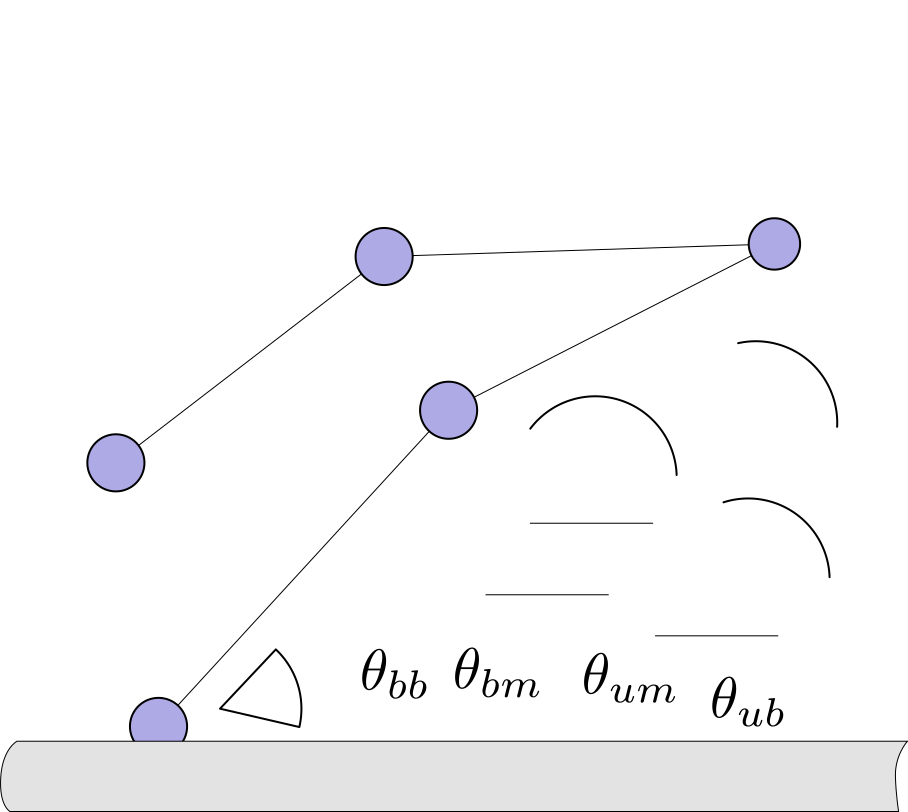
\includegraphics[width=.65\textwidth,keepaspectratio]{../figures/ob_fig}
%%   \caption{Onebound dynein model.}{}
%%   \label{fig:model-intro}
%% \end{figure}

\section{Model assumptions}
\subsection{Spherical domains connected by massless rods}
A key feature of the model is that each domain of the protein (two feet, two motors and a tail) is treated as a sphere. Each sphere is connected to one or two other spheres, as shown in Figure (\ref{fig:theory-intro}). This simplification is made to make the math easier and allow a simple definition of dynein's conformation.\\

As shown in Figure (\ref{fig:pdb-motm-dynein}), dynein's motor and tail domains are fairly spherical. Though the stalk and tail connecting these domains is definitely not massless, it is small enough that approximating it as massless should be reasonable. Making the radii of the spherical domains slightly larger should account for any drag caused by the rigid rods.\\

Each sphere has an associated drag factor $\gamma$, which describes the resistance it feels to motion. This drag factor is calculated based on the radius $R$ of the spheres, and is given by Stoke's Law:
%
\begin{equation}
  \gamma = 6\pi\nu R
\end{equation}
%
where this drag factor $\gamma$ is used later to calculate the velocity of each domain.\\

\subsection{Rods connecting domains are rigid}
The model assumes connected domains are rigidly attached to one another by rods. This assumption makes the math easier. One study found that the standard deviation of stalk and stem lengths in \textit{in vitro} dynein was roughly $1\text{nm}$ \cite{burgess-paper}. However a contrasting piece of evidence showed the coiled coil, a common protein structure which links the MTBD and motor domains in dynein, can stretch in myosin, another motor protein, by 2.5x \cite{myosin-cc-elasticity}. Another dynein simulation done by Sarlah \textit{et. al.} models the dynein stalk as an elastic rod \cite{sarlahmodel}.\\

In defense of rigid rods, the timescale of harmonic stalk oscillations is likely much quicker than that of the mechanochemical cycle, so it is reasonable to model the stalk as a rigid rod at the stalk's average extension length. Either way, it is then an assumption of the model that inter-domain elasticity is not necessary for stepping.\\

\subsection{Angular springs}
Each domain has a spring constant $c_b, c_m$ or $c_t$, for binding, motor or tail domains respectively, which decides the energy associated with that domain angle. For example, the tail domain energy is given by
%
\begin{equation}
  \Delta G_t = \frac12c_t\left(\theta_t - \theta_t^{eq}\right)^2
\end{equation}
%
This energy represents the conformational energy of that particular domain. This energy can be used to calculate a return force which pushes the domain back to equilibrium. A depiction of this is shown in Figure (\ref{fig:angular-spring}).\\

\begin{figure}[h]
  \centering
  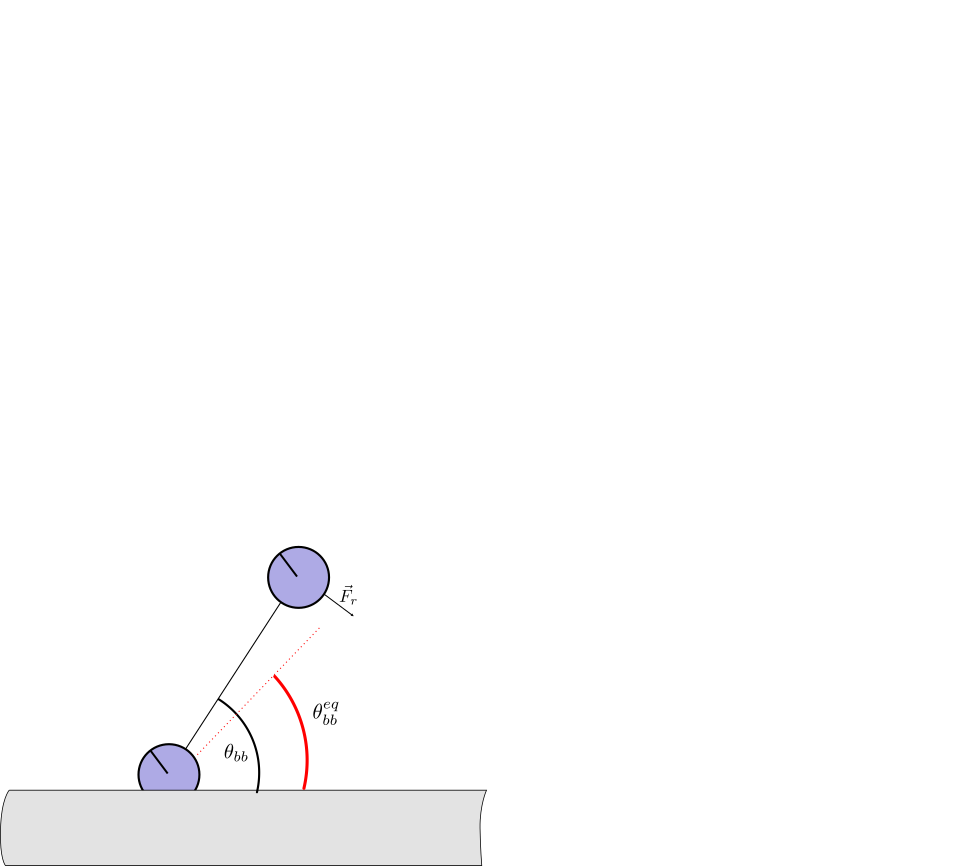
\includegraphics[width=.65\textwidth]{../figures/angular-spring}
  \caption{Angular spring return force when out of equilibrium.}{The $\theta_{bb}$ angle shown is greater than the equilibrium angle $\theta_{bb}^{eq}$, and thus the $bb$ domain has conformational energy $\frac{1}{2}c_b\left(\theta_{bb}-\theta_{bb}^{eq}\right)^2$, and feels a force pulling the motor domain towards the microtubule.}
  \label{fig:angular-spring}
\end{figure}

\subsection{Two-state model}
According to the Cianfrocco model, dynein takes on a total of eight states during a single step. Many of these states are conformationally very similar, e.g. the ADP- vs apo-bound or ATP- vs ADP-bound. Others involve quick transitions, e.g. from the just-MT-bound state to the post-powerstroke state. The transitions which take the most time according to reaction rate calculations are MT-binding and MT-release \cite{sarlahmodel}. Thus, these two states are taken to be the most important, and the Cianfrocco model is approximated by transitioning between these two states.\\

The main difference between these two states is that onebound has one diffusing MTBD, whereas bothbound has both its MTBDs MT-bound. Another key difference is equilibrium angles of the motor domains. During powerstroke, according to the Cianfrocco model, the dynein linker shifts, causing the tail-MTBD angle to shift. In this model, the conformation change caused by ATP hydrolysis is modelled as shifting the bothbound equilibrium angle $\theta_{xm}^{bb,eq}$ to $\theta_{xm}^{ob,eq}$.\\

\subsection{Transitioning between states}
The model transitions between states with a probability dependent on both the conformational energy difference between the two states and the physical separation between the MT and binding MTBD. This transition can be tricky. To unbind, or convert from a bothbound to onebound model, a onebound structure can be constructed with the exact same domain positions, except the unbound MTBD is allowed to diffuse. To bind, or convert from a onebound to bothbound model, the unbound MTBD must be projected onto the microtubule. This is because the bothbound state is defined as having both MTBDs at $y=0$. Once projected, a bothbound model can be constructed with domains in the same places as the projected onebound model.\\

The rates of such transitions are based on the conformational energy change between the new and old states. The energy difference between states A and B is given by:
%
\begin{equation}
  \Delta G_{A\rightarrow B} = \sum_{i=0...N_B}^{B} \frac{1}{2}c_i\left(\theta_i-\theta_i^B\right)^2 - \sum_{j=0...N_A}^{A} \frac{1}{2}c_j\left(\theta_j-\Theta_j^A\right)^2
\end{equation}
%
where B is the transitioned version of state A. Transition energies are used to calculate transition rates, as given by the Arhennius equation $k=Ae^{-\beta\Delta G}$, where $\beta = (k_BT)^{-1}$. In this equation $\Delta G$ is the total energy of transition between states and A is a constant known as the preexponential factor with units of $s^{-1}$.\\
%
\begin{equation}
  k_b = Ae^{-\beta\Delta G} = Ae^{-\beta\Delta G_{conf}}e^{-\beta\Delta G_{bind}}
\end{equation}
%
where $\Delta G_{conf}$ is the change in spring energy in going from bothbound to onebound and $\Delta G_{bind}$ is the energy gained from binding to the microtubule. Because binding energy for the MT-MTBD complex is hard to find, the following substitution is made:
%
\begin{equation}
  k_b = Ae^{\frac{-\Delta G}{k_BT}} = Be^{\frac{-\Delta G_{conf}}{k_BT}}
\end{equation}
%
Thus the transition rate is only dependent on the change in conformational energy of transitioning and the preexponential factor $B$. To prevent binding events from happening when the MTBD is high above the MT, the following step function correction is added to the rate equation: \\

\begin{equation}
  k_b = Be^{\frac{-\Delta G_{conf}}{k_BT}}\left(1-H\left(X_{uby}-0.1\right)\right)
\end{equation}

where H is the Heaviside step function and $X_{uby}$ is the y position of the unbound MTBD. Thus the binding rate is zero when the unbound MTBD is over $0.1$nm from the MT.\\

\subsection{Brownian dynamics}
\label{sec:bd}
The Brownian dynamics equation describes the motion of high-drag objects which spend most of their time at terminal velocity, and is given by:
%
\begin{equation}
  \dot{x} = \frac{1}{\gamma}\left(F_{net} + R\right)
\end{equation}
%
where $\gamma$ is the drag constant of the object and $R$ is a random Brownian force which describes the effects of water particle collision. $R$ is a Gaussian-sampled zero-centered force with variance given by:
%
\begin{equation}
  R_{\sigma^2} = \sqrt{\frac{2k_bT\gamma}{\delta t}}
\end{equation}
%
which is calculated from the Einstein relation.\\

\subsection{Binding to microtubule}
The model ``steps'' whenever an MTBD diffuses near the microtubule. \textit{in vivo}, dynein binds to a site on the $\alpha-\beta$ tubulin polymer microtubule which repeats roughly every 8nm. Thus, all dynein steps should be multiples of $8$nm. This model ignores this requirement and allows stepping to occur at any length. The assumption is that \textit{in vivo} dynein takes 8nm steps because it is tuned to take 8nm steps, not because it drags along the microtubule searching for a binding site. Thus the 8nm step length should be reproduced by the model even if stepping is allowed anywhere.\\

\subsection{2D model}
The coordinate system for this model is two-dimensional. Thus interactions between the two motors and MTBDs are ignored. This assumption is made to simplify the model. Other dynein models, like the winch model \cite{sarlahmodel}, add in attractive and repulsive forces between the two motors which act in three dimensions. This model ignores such effects.\\

\section{Deriving motion equations}
To simulate a protein's passage through the above mechanochemical cycle, equations are needed to describe the position of dynein at an arbitrary time. Using Euler's method, a position equation can be found given a velocity equation like so:

\begin{align}
  f(t+\delta t) &= f(t)+f'(t)\delta t
\end{align}

Thus, if velocity equations can be found for the individual domains, then dynein's dynamic behavior can be solved for using numerical integration. The Brownian dynamics equation shown in Section (\ref{sec:bd}) provides velocity at time t from forces at time t. All that needs to be done is to come up with expressions for the forces on each domain, which is done in the next two sections.\\

One complication arises from the choice of coordinate system. Angular coordinates are nice, since they automatically enforce the rigid rod constraint. However, forces are more easily calculated in Cartesian coordinates. In addition, forces on the $ith$ domain depend on domains $i\pm1$. Thus, solving for forces requires solving a large system of equations. Mathematica is used for this purpose, as outlined below.\\

\subsection{Prestroke onebound model}
Prestroke dynein is referred to as onebound, since one motor domain is bound to the MT in this state, and the other unbound. A spatial representation of onebound dynein is shown in Figure (\ref{fig:derivation-onebound}).

\begin{figure}[h]
  \centering
  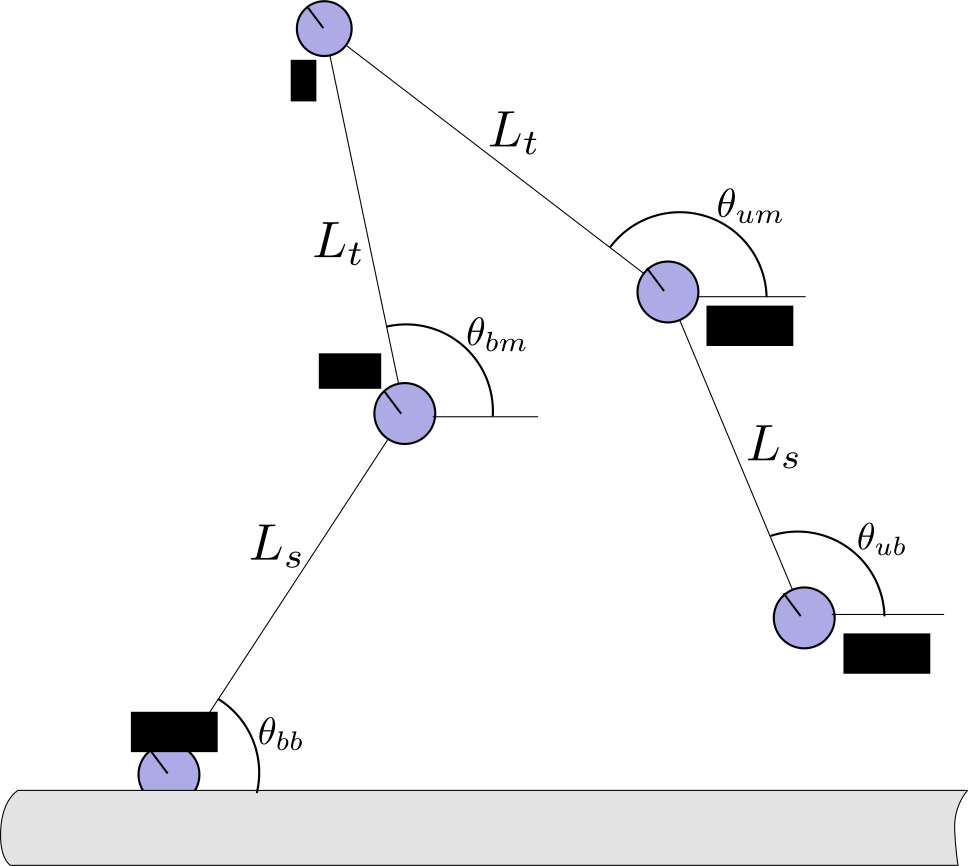
\includegraphics[width=.45\textwidth]{../figures/derivation-onebound}
  \caption{Spatial representation of the onebound dynein model.}{The coordinate system used for derivation of onebound forces.}
  \label{fig:derivation-onebound}
\end{figure}

The coordinate system for this model is as follows. The bound MTBD is referred to as the ``bound binding domain'' $bb$. Its coordinates take the form, for example, $X_{bb}$. The motor domain adjacent to $bb$ is the ``bound motor'' $bm$. Next is the tail $t$, then the ``unbound motor'' $um$ and finally $ub$.\\

The four angles $\theta_{bb}, \theta_{bm}, \theta_{um}$ and $\theta_{ub}$, corresponding to bound binding, bound motor, unbound motor and unbound binding angle, together describe any possible conformation the system can take on. The domain of $\theta_{bb}$ has a restricted domain of $[0,\pi]$ to prevent below-MT conformations, but the other angles have domains of $[0,2\pi]$. Each angle is defined relative to the horizontal axis. The position of the bound binding domain $X_{bb}$ and the four domain angles are all that is needed to determine the position of the protein at any time.\\

\subsubsection{Onebound velocity calculations}

The following equations allow recursive calculation of the positions of each domain in Cartesian coordinates:

\noindent\begin{minipage}{0.49\linewidth}
\begin{align}
  X_{bm} &= X_{bb}+L_{s}\cos(\theta_{bb}) \\
  X_{t}  &= X_{bm}+L_{t}\cos(\theta_{bm}) \\
  X_{fm} &= X_{t} - L_{t}\cos(\theta_{fm}) \\
  X_{fb} &= X_{fm} - L_{s}\cos(\theta_{fb})
\end{align}
\end{minipage}
\begin{minipage}{0.49\linewidth}
\begin{align}
  Y_{bb} &= 0 \\
  Y_{bm} &= Y_{bb}+L_{s}\sin(\theta_{bb}) \\
  Y_{t}  &= Y_{bm}+L_{t}\sin(\theta_{bm}) \\
  Y_{fm} &= Y_{t} - L_{t}\sin(\theta_{fm}) \\
  Y_{fb} &= Y_{fm} - L_{s}\sin(\theta_{fb})
\end{align}
\end{minipage}
\vspace{.5cm}

$L_s$ and $L_t$ correspond to lengths of each interdomain rod, and the $t$ subscripts refer to tail domain coordinates.\\

The goal is to express angular velocities $\dot{\theta}_{bb}, \dot{\theta}_{bb}, \dot{\theta}_{bb}$ and $\dot{\theta}_{bb}$ in terms of known quantities. To begin, the Cartesian velocities of each domain can be calculated from the above position equations in a similar recursive manner. A subset of the equations are shown here:

\noindent\begin{minipage}{0.49\linewidth}
\begin{align}
  \dot{X}_{bb} &= 0 \\
  \dot{X}_{bm} &= \dot{X}_{bb} - L_{s}\sin(\theta_{bb})\dot{\theta}_{bb} \label{cartesian-bmx}\\
  \dot{X}_{t } &= \dot{X}_{bm} - L_{t}\sin(\theta_{bm})\dot{\theta}_{bm}
  %% \dot{X}_{fm} &= \dot{X}_{t } + L_{t}\sin(\theta_{fm})\dot{\theta}_{fm} \\
  %% \dot{X}_{fb} &= \dot{X}_{fm} + L_{s}\sin(\theta_{fb})\dot{\theta}_{fb}
\end{align}
\end{minipage}
\begin{minipage}{0.49\linewidth}
\begin{align}                                                                          
  \dot{Y}_{bb} &= 0 \\                                                        
  \dot{Y}_{bm} &= \dot{Y}_{bb} + L_{s}\cos(\theta_{bb})\dot{\theta}_{bb} \\
  \dot{Y}_{t}  &= \dot{Y}_{bm} + L_{t}\cos(\theta_{bm})\dot{\theta}_{bm}
  %% \dot{Y}_{fm} &= \dot{Y}_{t } - L_{t}\cos(\theta_{fm})\dot{\theta}_{fm} \\
  %% \dot{Y}_{fb} &= \dot{Y}_{fm} - L_{s}\cos(\theta_{fb})\dot{\theta}_{fb}
\end{align}
\end{minipage}
\vspace{.5cm}

Another way to express these Cartesian velocities is using the Brownian dynamics equation $\dot{X} = \frac1\gamma F_{net} + R$:

\begin{align}  
  \dot{X}_{bm} &= \frac{1}{\gamma_m} \Big(F_{xml} + - \lambda_{bs}(X_{bm} - X_{bb}) + \lambda_{bt}(X_{t } - X_{bm}) \Big) + R_{xml} \label{brownian-bmx}\\
  \dot{X}_{t } &= \frac{1}{\gamma_t} \Big(F_{xt } + - \lambda_{bt}(X_{t } - X_{bm}) + \lambda_{ft}(X_{fm} - X_{t }) \Big) + R_{xt }
  %% \dot{X}_{fm} &= \frac{1}{\gamma_m} \Big(F_{xmr} + - \lambda_{ft}(X_{fm} - X_{t }) + \lambda_{fs}(X_{fb} - X_{fm}) \Big) + R_{xmr} \\
  %% \dot{X}_{fb} &= \frac{1}{\gamma_b} \Big(F_{xbr} + - \lambda_{fs}(X_{fb} - X_{fm}) \Big) + R_{xbr}
\end{align}
%
where $\gamma_n$ is a drag coefficient for the binding, motor or tail domain with units of mass per second. $F_{xn}$ is the x component of external force on each domain $n$ due to various factors. $\lambda_{12}\left(X_1 - X_2\right)$ is the x component of internal force on domain $2$ due to domain $1$, where $\lambda$ is a tension coefficient with units of mass per second squared, also known as a Lagrange multiplier. $R_{xn}$ is the Brownian coefficient representing motion due to solvent collision, with units of velocity.\\

These two sets of equations, Cartesian and Brownian, can be equated to get more interesting equations. For example, Eq (\ref{cartesian-bmx}) and Eq (\ref{brownian-bmx}) can be equated. This equating, combined with expanding the recursive velocity definitions leads to new equations, some of which are shown here:

\begin{align}
  &-L_s\sin(\theta_{bb})\dot{\theta}_{bb} = \frac{1}{\gamma_m}F_{xml} + -\frac{1}{\gamma_m}\lambda_{bs}(X_{bm} - X_{bb}) + \frac{1}{\gamma_m}\lambda_{bt}(X_{t } - X_{bm}) + R_{bmx} \label{ob_system_first}\\
  &-L_s\sin(\theta_{bb})\dot{\theta}_{bb} - L_t\sin(\theta_{bm})\dot{\theta}_{bm} = \frac{1}{\gamma_t}F_{xt } + -\frac{1}{\gamma_t}\lambda_{bt}(X_{t } - X_{bm}) + \frac{1}{\gamma_t}\lambda_{ft}(X_{um} - X_{t }) + R_{tx}\label{ob_system_second}
\end{align}
%
A total of eight coupled differential equations are formed from this procedure. These eight equations form a system of equations with eight unknowns: $\dot{\theta}_{bb}, \dot{\theta}_{bb}, \dot{\theta}_{bb}$ and $\dot{\theta}_{bb}$, and the four tension coefficients $\lambda_{bs}, \lambda_{bt}, \lambda_{um}$ and $\lambda_{ub}$. This system is more compactly represented as:
{\small
  \[
  \hspace{-1.0cm}
  \resizebox{0.85\linewidth}{!}{%
  $\begin{pmatrix}
    L_s\sin\theta_{bb} & 0 & 0 & 0 & -\gamma_m (X_{bm} - X_{bb}) & \gamma_m (X_{t } - X_{bm}) & 0 & 0\\
    L_s\sin(\theta_{bb}) & L_t\sin(\theta_{bm}) & 0 & 0 & 0 & -\gamma_t (X_{t } - X_{bm}) & \gamma_t (X_{um} - X_{t }) & 0\\
    L_s\sin(\theta_{bb}) & L_t\sin(\theta_{bm}) & -L_t\sin(\theta_{um}) & 0 & 0 & 0 & -\gamma_m (X_{um} - X_{t }) & \gamma_m (X_{ub} - X_{um})\\
    L_s\sin(\theta_{bb}) & L_t\sin(\theta_{bm}) & -L_t\sin(\theta_{um}) & -L_s\sin(\theta_{ub}) & 0 & 0 & 0 & -\gamma_b (X_{ub} - X_{um})\\
    -L_s\cos(\theta_{bb}) & 0 & 0 & 0 & -\gamma_m (Y_{bm} - Y_{bb}) & \gamma_m (Y_{t } - Y_{bm}) & 0 & 0\\
    -L_s\cos(\theta_{bb}) & -L_t\cos(\theta_{bm}) & 0 & 0 & 0 & -\gamma_t (Y_{t } - Y_{bm}) & \gamma_t (Y_{um} - Y_{t }) & 0\\
    -L_s\cos(\theta_{bb}) & -L_t\cos(\theta_{bm}) & L_t\cos(\theta_{um}) & 0 & 0 & 0 & -\gamma_m (Y_{um} - Y_{t }) & \gamma_m (Y_{ub} - Y_{um})\\
    -L_s\cos(\theta_{bb}) & -L_t\cos(\theta_{bm}) & L_t\cos(\theta_{um}) & L_s\cos(\theta_{ub}) & 0 & 0 & 0 & -\gamma_b (Y_{ub} - Y_{um})\\
  \end{pmatrix}$%
  }
  \begin{pmatrix}
    \dot{\theta}_{bb}\\
    \dot{\theta}_{bm}\\
    \dot{\theta}_{um}\\
    \dot{\theta}_{ub}\\
    \lambda_{bs}\\
    \lambda_{bt}\\
    \lambda_{ut}\\
    \lambda_{us}\\
  \end{pmatrix}
  =
  \begin{pmatrix}
    -F_{bmx} + \gamma_m R_{bmx}\\
    -F_{tx} + \gamma_t R_{tx}\\
    -F_{umx} + \gamma_m R_{umx}\\
    -F_{ubx} + \gamma_b R_{ubx}\\
    -F_{bmy} + \gamma_m R_{bmy}\\
    -F_{ty} + \gamma_t R_{ty}\\
    -F_{umy} + \gamma_m R_{umy}\\
    -F_{uby} + \gamma_b R_{uby}\\
  \end{pmatrix}
  \]
}

This matrix is then solved using the Mathematica computer algebra system, resulting in a set of motion equations which describe the model's trajectory over time, e.g. $\dot{\theta_{bm}}(\theta_{bb}, \theta_{bm}, \theta_{um}, \theta_{ub})$. These motion equations are further described in Appendix (\ref{sec:AppendixOneboundEquations}).\\

\subsection{Poststroke bothbound model}
The main difference between the prestroke and poststroke mathematical models is that the latter has a further constraint: both of its MTBDs are attached to the MT. This has the effect of diminishing the degrees of freedom of the system from four to two, assuming the motor remains above the MT. A spatial representation of the bothbound model is shown in Figure (\ref{fig:derivation-bothbound}).\\

\begin{figure}[h]
  \centering
  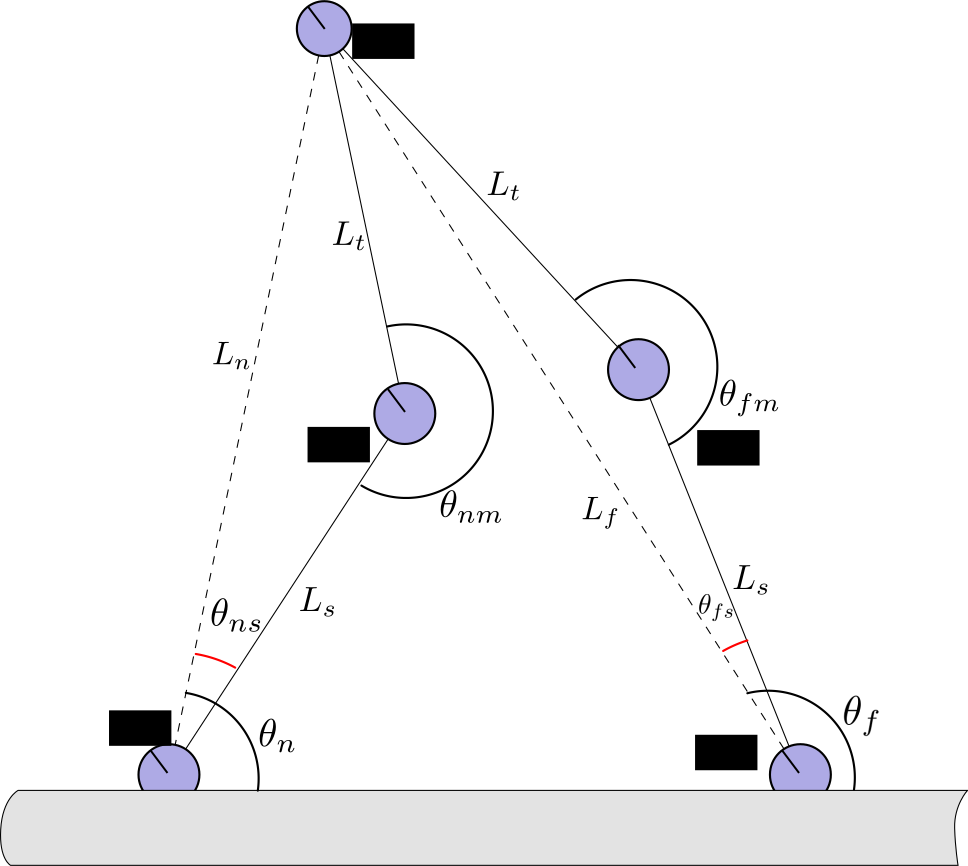
\includegraphics[width=.45\textwidth]{../figures/derivation-bothbound}
  \caption{Spatial representation of the bothbound dynein model.}{The coordinate system used for derivation of bothbound forces.}
  \label{fig:derivation-bothbound}
\end{figure}

The main differences between onebound and bothbound are the naming scheme and spatial constraints. Dimers can no longer be differentiated by being un/bound, so are now differentiated by their z-position: being near or far from the ``camera.'' This is similar to labeling them as the right or left dimer. Thus there is the near binding domain $nb$, near motor $\text{nm}$, tail $t$, far motor $fm$ and far binding domain $fb$. Both the near and far binding domains have their y-coordinate fixed at zero. The system is described completely by two angles: $\theta_{nm}$ and $\theta_{fm}$. Angles $\theta_t, \theta_{nb}$ and $\theta_{fb}$ are dependent on these two motor angles. Intermediate variables $L_{n}$ and $L_{f}$ are computed to ease calculations. The second MTBD constraint adds another required piece of information the model must track: the x position of the second MTBD. This position is described by $L$, the displacement between the near and far binding domains.\\

\subsubsection{Bothbound velocity calculations}

The first step in calculating angular velocities is to define intermediate variables $L_n$ and $L_f$ using the law of cosines:

\begin{align}
  L_n &= \sqrt{L_s^2 + L_t^2 - 2L_sL_t\cos{\theta_{nm}}} \\
  L_f &= \sqrt{L_s^2 + L_t^2 - 2L_sL_t\cos{\theta_{fm}}}
\end{align}

These new artificial stalks are not physically relevant, but allow the definition of new angles $\theta_n, \theta_{ns}, \theta_{f}$ and $\theta_{fs}$, which are useful for calculating the position of the motor domain. The treatment of the near and far versions of these angles is very similar, so only the near angles will be dealt with here. The angles themselves are never dealt with, only their sines and cosines:

\begin{align}
  \cos\theta_n &= \frac{L^2 + L_n^2 - L_f^2}{2L L_n} \\
  \sin\theta_{n} &= \sqrt{1 - \cos^2\theta_{n}} \\
  \cos\theta_{ns} &= \frac{L_s^2 + L_n^2 - L_t^2}{2L_s L_n} \\
  \sin\theta_{ns} &=
  \begin{cases}
    +\sqrt{1 - \cos^2\theta_{ns}} & \theta_{nm} < \pi \\
    -\sqrt{1 - \cos^2\theta_{ns}} & \theta_{nm} > \pi
  \end{cases}
\end{align}

These values are arrived at through the Law of Cosines and a trigonometric identity. The sign of $\sin\left(\theta_n\right)$ is restricted to positive values due to the angle's $[0,\pi]$ domain. $\theta_{ns}$'s domain is $[-\pi,\pi]$, meaning its sign is not restricted. The partial derivatives of these values are used in future calculations, and some are shown here:

\begin{align}
  \frac{\partial \cos\theta_n}{\partial L_n} &= \frac{1}{L} - \frac{L^2 + L_n^2 - L_f^2}{2L L_n^2}\\
  \frac{\partial \cos\theta_n}{\partial L_f} &= -\frac{L_f}{LL_n}\\
  \frac{\partial \sin\theta_n}{\partial L_n} &= \frac{-\cos\theta_n}{\sqrt{1-\cos^2\theta_n}}
  \left(\frac{1}{L} - \frac{L^2 + L_n^2 - L_f^2}{2L L_n^2}\right)
  %% \frac{\partial \sin\theta_n}{\partial L_f} &= \frac{-\cos\theta_n}{\sqrt{1-\cos^2\theta_n}}
  %% \left(\frac{-L_f}{LLn}\right)\\
  %% \frac{\partial \cos\theta_{ns}}{\partial L_n} &= \frac{1}{L_s}
  %% - \frac{L_s^2 + L_n^2 - L_t^2}{2L_sL_n^2}\\
  %% \frac{\partial \cos\theta_{ns}}{\partial L_f} &= 0\\
  %% \frac{\partial \sin\theta_{ns}}{\partial L_n} &=
  %% \begin{cases}
  %%   \frac{-\cos\theta_{ns}}{\sqrt{1-\cos^2\theta_{ns}}}
  %%   \left(\frac{1}{L_s} - \frac{L_s^2+L_n^2-L_t^2}{2LL_n^2}\right) & \theta_{nm} < \pi \\
  %%   \frac{\cos\theta_{ns}}{\sqrt{1-\cos^2\theta_{ns}}}
  %%   \left(\frac{1}{L_s} - \frac{L_s^2+L_n^2-L_t^2}{2LL_n^2}\right) & \theta_{nm} > \pi
  %% \end{cases}\\
  %% \frac{\partial \sin\theta_{ns}}{\partial L_f} &= 0
\end{align}
%
The position of the motor and tail domains is calculated as follows, using the angle addition trigonometric identity:

\begin{align}
  X_{nm} &= L_s\left(
  \cos\theta_n\cos\theta_{ns} - \sin\theta_n\sin\theta_{ns}
  \right)
  \\
  Y_{nm} &= L_s\left(
  \cos\theta_n\sin\theta_{ns} + \sin\theta_n\cos\theta_{ns}
  \right)
  \\
  X_{t} &= L_n\cos\theta_n\\
  Y_{t} &= L_n\sin\theta_n
\end{align}

The partial derivatives of these values are used later. A selection are shown here:

\begin{align}
  \frac{dX_{nm}}{dL_n} &= L_s\Big(\cos\theta_n\frac{d\cos\theta_{ns}}{dL_n} + \cos\theta_{ns}\frac{d\cos\theta_{n}}{dL_n} - \sin\theta_n\frac{d\sin\theta_{ns}}{dL_n} - \sin\theta_{ns}\frac{d\sin\theta_{n}}{dL_n}\Big)\\
  \frac{dY_{nm}}{dL_n} &= L_s\Big(\cos\theta_n\frac{d\sin\theta_{ns}}{dL_n} + \sin\theta_{ns}\frac{d\cos\theta_{n}}{dL_n} + \sin\theta_n\frac{d\cos\theta_{ns}}{dL_n} + \cos\theta_{ns}\frac{d\sin\theta_{n}}{dL_n} \Big)\\
  \frac{dX_{nm}}{dL_f} &= L_s\Big(\cos\theta_n\frac{d\cos\theta_{ns}}{dL_f} + \cos\theta_{ns}\frac{d\cos\theta_{n}}{dL_f} - \sin\theta_n\frac{d\sin\theta_{ns}}{dL_f} - \sin\theta_{ns}\frac{d\sin\theta_{n}}{dL_f} \Big)
  %% \frac{dY_{nm}}{dL_f} &= L_s\Big(\cos\theta_n\frac{d\sin\theta_{ns}}{dL_f} + \sin\theta_{ns}\frac{d\cos\theta_{n}}{dL_f} + \sin\theta_n\frac{d\cos\theta_{ns}}{dL_f} + \cos\theta_{ns}\frac{d\sin\theta_{n}}{dL_f}\Big)\\
  %% \frac{dX_{t}}{dL_n} &= \cos\theta_n + L_n\frac{\partial \cos\theta_n}{\partial L_n} = \frac{L_n}{L}\\
  %% \frac{dY_{t}}{dL_n} &= \sin\theta_n + L_n\frac{\partial \sin\theta_n}{\partial L_n}\\
  %% \frac{dX_{t}}{dL_f} &= L_n\frac{\partial \cos\theta_n}{\partial L_f} = -\frac{L_f}{L}\\
  %% \frac{dY_{t}}{dL_f} &= L_n\frac{\partial \sin\theta_n}{\partial L_f}\\
\end{align}
%
These partial derivatives are then used in a system of equations very similar to that in Equations (\ref{ob_system_first}-\ref{ob_system_second}), combining Brownian and coordinate system definitions of domain velocities:

\begin{align}
  \dot{X}_{nm} &= \frac{1}{\gamma} \Big(F_{xml} - \lambda_{ns}(X_{bm} - X_{bb})
  + \lambda_{nt}(X_{t } - X_{bm}) \Big) + R_{xml}
  &=& \frac{\partial X_{nm}}{\partial L_n}\dot{L}_n + \frac{\partial X_{nm}}{\partial L_f}\dot{L}_f\\
  \dot{X}_{t } &= \frac{1}{\gamma} \Big(F_{xt } - \lambda_{nt}(X_{t } - X_{bm})
  + \lambda_{ft}(X_{fm} - X_{t }) \Big) + R_{xt }
  &=& \frac{\partial X_{t}}{\partial L_n}\dot{L}_n + \frac{\partial X_{t}}{\partial L_f}\dot{L}_f\\
  \dot{X}_{fm} &= \frac{1}{\gamma} \Big(F_{xmr} - \lambda_{ft}(X_{fm} - X_{t })
  + \lambda_{fs}(X_{fb} - X_{fm}) \Big) + R_{xmr}
  &=& \frac{\partial X_{fm}}{\partial L_n}\dot{L}_n + \frac{\partial X_{fm}}{\partial L_f}\dot{L}_f
\end{align}

\begin{align}
  \dot{Y}_{nm} &= \hspace{1cm} \frac{1}{\gamma} \Big(F_{yml} - \lambda_{ns}(Y_{bm} - Y_{bb})
  + \lambda_{nt}(Y_{t } - Y_{bm}) \Big) + R_{yml}
  &= \frac{\partial Y_{nm}}{\partial L_n}\dot{L}_n + \frac{\partial Y_{nm}}{\partial L_f}\dot{L}_f\\
  \dot{Y}_{t}  &= \hspace{1cm} \frac{1}{\gamma} \Big(F_{yt } - \lambda_{nt}(Y_{t } - Y_{bm})
  + \lambda_{ft}(Y_{fm} - Y_{t }) \Big) + R_{yt }
  &= \frac{\partial Y_{t}}{\partial L_n}\dot{L}_n + \frac{\partial Y_{t}}{\partial L_f}\dot{L}_f\\
  \dot{Y}_{fm} &= \hspace{1cm} \frac{1}{\gamma} \Big(F_{ymr} - \lambda_{ft}(Y_{fm} - Y_{t })
  + \lambda_{fs}(Y_{fb} - Y_{fm}) \Big) + R_{ymr}
  &= \frac{\partial Y_{fm}}{\partial L_n}\dot{L}_n + \frac{\partial Y_{fm}}{\partial L_f}\dot{L}_f
\end{align}
%
The matrix version of this system looks like:

\[
\begin{pmatrix}
  -\frac{X_{nm}}{Ln} & -\frac{X_{nm}}{Lf}
  & -\frac{X_{nm}-X_{nb}}{\gamma} & \frac{X_{t}-X_{nm}}{\gamma} & 0 & 0\\
  -\frac{X_{t}}{Ln} & -\frac{X_{t}}{Lf}
  & 0 & -\frac{X_{t}-X_{nm}}{\gamma} & \frac{X_{fm}-X_{t}}{\gamma} & 0\\
  -\frac{X_{fm}}{Ln} & -\frac{X_{fm}}{Lf}
  & 0 & 0 & -\frac{X_{fm}-X_{t}}{\gamma} & \frac{X_{fb}-X_{fm}}{\gamma}\\
  -\frac{Y_{nm}}{Ln} & -\frac{Y_{nm}}{Lf}
  & -\frac{Y_{nm}-Y_{nb}}{\gamma} & \frac{Y_{t}-Y_{nm}}{\gamma} & 0 & 0\\
  -\frac{Y_{t}}{Ln} & -\frac{Y_{t}}{Lf}
  & 0 & -\frac{Y_{t}-Y_{nm}}{\gamma} & \frac{Y_{fm}-Y_{t}}{\gamma} & 0\\
  -\frac{Y_{fm}}{Ln} & -\frac{Y_{fm}}{Lf}
  & 0 & 0 & -\frac{Y_{fm}-Y_{t}}{\gamma} & \frac{Y_{fb}-Y_{fm}}{\gamma}\\
\end{pmatrix}
\begin{pmatrix}
  \dot{L}_n\\
  \dot{L}_f\\
  \lambda_{ns}\\
  \lambda_{nt}\\
  \lambda_{ft}\\
  \lambda_{fs}\\
\end{pmatrix}
=
\begin{pmatrix}
  -\frac{1}{\gamma}F_{nmx} - R_{nmx}\\
  -\frac{1}{\gamma}F_{tx}  - R_{tx}\\
  -\frac{1}{\gamma}F_{fmx} - R_{fmx}\\
  -\frac{1}{\gamma}F_{nmy} - R_{nmy}\\
  -\frac{1}{\gamma}F_{ty}  - R_{ty}\\
  -\frac{1}{\gamma}F_{fmy} - R_{fmy}\\
\end{pmatrix}
\]
%
This system of equations is then solved and used to calculate $\dot{L}_n$ and $\dot{L}_f$, as shown in Appendix (\ref{sec:AppendixBothboundEquations}). These intermediate velocities can then be used to calculate $\dot{\theta_{nm}}$ and $\dot{\theta_{fm}}$.\\

%% \subsection{Converting experimental rates to preexponential factors $A_b$ and $A_{ub}$}
%% Rate constants $k_b$ and $k_{ub}$ govern the probability of transitioning from onebound to bothbound and vice-versa, respectively. One issue is that when these parameters are measured experimentally, the values represent the average rate for an ensemble of dynein in many different conformations. In contrast, the rates the model uses represent the probability of unbinding of a specific conformation. Thus, it is necessary to find a way to convert between experimental rates $k_b^{exp}$ and $k_{ub}^{exp}$ and conformation-specific rates $k_b$ and $k_{ub}$. As shown in Section \ref{sec:transitioning-states}, rates can be expressed using the Arrhenius equation:

%% \begin{align*}
%%   k_b &= A_b'e^{\frac{-\Delta G_{bind}}{k_BT}} = A_b'e^{\frac{-\Delta G_{conf}^{ob\rightarrow bb}}{k_BT}}e^{\frac{-\Delta G_{bind}}{k_BT}} = A_be^{\frac{-\Delta G_{conf}^{ob\rightarrow bb}}{k_BT}}\\
%%   k_{ub} &= A_{ub}'e^{\frac{-\Delta G_{unbind}}{k_BT}} = A_{ub}'e^{\frac{-\Delta G_{conf}^{bb\rightarrow ob}}{k_BT}}e^{\frac{\Delta G_{bind}}{k_BT}} = A_{ub}e^{\frac{-\Delta G_{conf}^{bb\rightarrow ob}}{k_BT}}
%% \end{align*}

%% where the constant Boltzmann factor for binding energy are hidden inside the unprimed preexponential factors. The experimental values are calculated the same way, with the free energy changes replaced with expectation values. Since by the equipartition theorem $\left<G_{conf}^{ob}\right> = 2k_BT$ and $\left<G_{conf}^{bb}\right> = k_BT$, the equations can be simplified:

%% \begin{align*}
%%   k_b^{exp} &= A_be^{\frac{-\left(2k_BT - k_BT\right)}{k_BT}} = \frac{A_b}{e}\\
%%   k_{ub}^{exp} &= A_{ub}e^{\frac{-\left(k_BT-2k_BT\right)}{k_BT}} = A_{ub}e
%% \end{align*}

%% Thus experimental rates can be converted easily into the model parameters $A_b$ and $A_{ub}$.

%% \subsection{Literature values for experimental binding rates}
%% Sarlah \textit{et. al.} \cite{sarlahmodel} perform a similar simulation of dynein and provide the reaction rates shown in Figure \ref{fig:sarlah-rate-table}.

%% \begin{figure}[h]
%%   \centering
%%   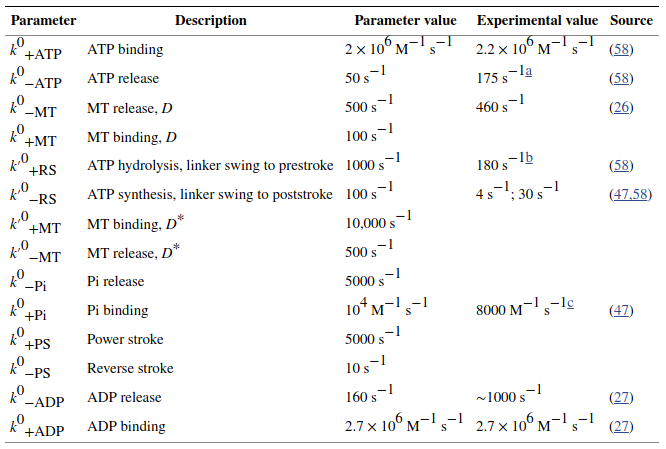
\includegraphics[width=.45\textwidth]{../figures/SarlahParameterTable.png}
%%   \caption{Sarlah kinetic rates.}{Kinetic rates used in Sarlah \textit{et. al.}'s model \cite{sarlahmodel}.}
%%   \label{fig:sarlah-rate-table}
%% \end{figure}

%% The assumption of this project is that many of the states in this table can be combined into a single state without loss of predictive power of dynein behavior. Specifically, the assumption is that ejecting phosphate, conducting the powerstroke, releasing ADP, binding ATP and dissociating from the microtubule and all occur during the bothbound state, and hydrolyzing ATP, conducting the prestroke and rebinding the MT occur during onebound. These states are roughly grouped as MT-bound and MT-unbound states in the Cianfrocco mechanochemical cycle \cite{cianfroccoreview}.\\

%% The rate-limiting transitions in the Cianfrocco model are used as the guess $k_b$ and $k_{ub}$ values. That means that, since ATP hydrolysis has the slowest rate constant in onebound and MT release has the slowest rate in bothbound, $k_b^{exp} = 180 s^{-1}$ and $k_{ub} = 460 s^{-1}$ serve as good initial guesses.\\

\newpage
\chapter{Methods}
\label{chap:Methods}
This section will go into detail on how the model was implemented in C++ and verified for accuracy and physicality.\\

\section{Simulation}
To generate stepping data, the models were coded in \verb|C++| and time-evolved using Euler's method to generate reasonable dynamical behavior. When in a position deemed worthy of a state transition, the model was converted to the respective other model, representing part of a ``step'' through the mechanochemical cycle.\\

\subsection{Time evolution}
Euler's method for solving differential equations was used to calculate domain positions through time. Because each model is a set of multiple coupled differential equations, care was taken to update each domain position at the same time, and not in a cascade. A code snippet is shown in Figure (\ref{snip:euler-code-snippet}) for the onebound updating scheme. This code calculates domain velocities for onebound dynein and uses them to find position displacements. These values are stored in temporary variables first, then updated all at once. The \verb|dt| used to update was $10^{-11}$ seconds.

\begin{figure}[h!]
  \centering
  \begin{tabular}{c}
    \begin{lstlisting}[language=python]
      def simulate(dyn_ob):
          t = 0
          while (t < runtime):
              double temp_bba = dyn_ob->get_bba() + dyn_ob->get_d_bba() * dt
              double temp_bma = dyn_ob->get_bma() + dyn_ob->get_d_bma() * dt
              double temp_uma = dyn_ob->get_uma() + dyn_ob->get_d_uma() * dt
              double temp_uba = dyn_ob->get_uba() + dyn_ob->get_d_uba() * dt
              
              dyn_ob->set_bba(temp_bba)
              dyn_ob->set_bma(temp_bma)
              dyn_ob->set_uma(temp_uma)
              dyn_ob->set_uba(temp_uba)
              
              t += dt
    \end{lstlisting}
  \end{tabular}
  \caption{Domain time evolution via Euler's method code snippet.}{}
  \label{snip:euler-code-snippet}
\end{figure}

\subsection{Transitioning between states}

\subsubsection{Transition rate}
\label{sec:transitioning-states}
Transitions from one state to another are accomplished by calculating the probability of a transition $t$ at a given timestep, given by $P_{t} = k_t\delta t$. Each timestep a value in $[0,1]$ is sampled from a random number generator and, if the roll is lower than $k_tdt$, the respective transition is made. The following sections describe how transitions are done.\\

\subsubsection{Onebound to bothbound transition calculation}
When binding occurs, conversion between OB and BB models is done by creating a bothbound dynein which is as similar in terms of domain position as possible to the onebound dynein.\\

Due to the nature of the simulation, binding attempts must occur above, but very close to, the microtubule. This is because \textit{in vivo}, electrostatic interactions between MTBD and MT bring the two together when they are near. These electrostatic interactions are not present in the model, and so are simulated by allowing binding attempts to occur when $Y_{ub} \leq 0.1\text{nm}$ above the MT. When a binding attempt is successful, the unbound binding domain of the OB dynein is ``teleported'' such that $Y_{ub} = 0.0$. This is to enforce the constraint that both binding domains of the BB model are directly on the MT.\\

To create a BB model from OB, the following intermediate variables are first computed:\\

\begin{align}
  L_n^2 &= \left(X_t - X_{nb}\right)^2 + Y_t^2\\
  L_f^2 &= \left(X_t - X_{fb}\right)^2 + Y_t^2\\
  \cos(\theta_{nm}) &= \frac{L_s^2 + L_t^2 - L_n^2}{2L_sL_t}\\
  \cos(\theta_{fm}) &= \frac{L_s^2 + L_t^2 - L_f^2}{2L_sL_t}
\end{align}

\subsubsection{Bothbound to onebound transition calculation}
Similar to the binding transition, unbinding involves creating a new onebound dynein from the old bothbound. To accomplish a transition to the farbound state, the following equations are used:

\begin{align}
  \theta_{new,bba} &= \theta_{old,nba}\\
  \theta_{new,bma} &= \theta_{old,nma} + \theta_{old,nba} - \pi\\
  \theta_{new,uma} &= \theta_{old,fma} + \theta_{old,fba} - \pi\\
  \theta_{new,uba} &= \theta_{old,fba}
\end{align}
%
To do a nearbound transition, the ``f'' and ``n'' subscripts in the above equations are swapped.\\

As shown in Section (\ref{table:thesis-parameters}), the MT binding rate is much quicker than the unbinding rate. This means that, when just unbound, the rate of rebinding is very high.\\

%% \subsection{Corrections}
%% \label{corrections-section}
%% Certain configurations of the model, such as in the bothbound model when $\theta_{nm} = \pi$ or $\theta_{fm} = \pi$, it becomes impossible to calculate intermediate variables due to values going to infinity (name for this??). For example when $\theta_{nm} = \pi$, $Ln = Ls + Lt$ and so:

%% \begin{align}
%%   \cos\theta_{ns} &= 1 \\
%%   \sin\theta_{ns} &= 0 \\
%%   \mbox{some val?} &\rightarrow \infty
%% \end{align}

%% Alternative problem states are when $L = 0$ and ???. These states are corrected similarly.\\

\subsection{Calculating forces}
Spring and Brownian forces are used to properly move the model through time. Appendices (\ref{sec:AppendixOneboundEquations}-\ref{sec:AppendixBothboundEquations}) show angular velocities are functions of the x- and y-components of both spring forces $F$ and Brownian forces $\gamma R$. Each Brownian force $R_{n,m}$ on domain $n$ in direction $m$ is sampled from a Gaussian with standard deviation $\sqrt{\frac{2k_BT\gamma_n}{dt}}$.\\

Spring forces are calculated by first finding the torque $\tau$ on each angle, then converting this to a force. For example, the onebound near motor angle feels a force $\tau_{nm} = c_m(\theta_{nm}-\theta_{nm,eq})$, where $c_n$ is the spring constant of the motor domain and $\theta_{nm,eq}$ the equilibrium angle. The magnitude of force on the adjacent binding and tail domains is thus $\tau/L_s$ and $\tau/L_t$, pointing in the direction adjacent the Ls and Lt rods, respectively. The force on the motor domain is found as the equal-and-opposite force to these two imposed forces. A sample calculation is shown in Snippet (\ref{snip:transition-rate-snippet}). Torque is calculated the near motor's angular displacement from equilibrium. This is converted to force exerted on adjacent domains. Finally, the equal and opposite force is exerted on the near motor domain.\\

\begin{figure}[h]
  \centering
  \begin{tabular}{c}
    \begin{lstlisting}[language=C++]
      def set_onebound_restoring_forces():
          T = cm*(nma - nma_eq);
          f1 = T/Ls;
          f2 = T/Lt;
          f1x = f1 * sin(bba);
          f1y = f1 * -cos(bba);
          f2x = f2 * sin(bma);
          f2y = f2 * -cos(bma);
          f.bbx += f1x;
          f.bby += f1y;
          f.tx  += f2x;
          f.ty  += f2y;
          f.bmx += -(f1x + f2x); // equal and opposite forces
          f.bmy += -(f1y + f2y);
    \end{lstlisting}
  \end{tabular}
  \caption{Code snippet of restoring force calculation.}{}
  \label{snip:transition-rate-snippet}
\end{figure}

\section{Verifying the model}
The models were verified to follow physical laws by checking their behavior in various tests: general conformational tests, energy conservation and obeying the equipartition theorem. The purpose of these tests was to verify that equations had been entered properly (primarily the conformational and energy conservation tests), and that the model obeyed the laws of physics (all tests).\\

A series of conformational tests were done to test if the coordinate systems of either model worked. These are listed in Appendix (\ref{sec:conformational-tests}).\\

\subsection{Energy conservation}
\label{sec:energy-conservation}
To verify that the magnitudes of forces are calculated properly, a conservation of energy test was performed. A very slight angular nudge was applied to either model. This nudge caused a small change in energy. This change in energy was compared with the work the forces on each domain caused over the nudge. For energy to be conserved, these values were required to be very similar. Mathematically the test required the following:

\begin{equation}
  \sum_n \frac12 \left(\theta_{nudge} - \theta_{n} - \theta_{n,eq}\right) = \sum_n \vec{F}_n \cdot \vec{r}_{n,nudge}
\end{equation}

where $\theta_{nudge}$ was the angular nudge applied, $F_n$ the net force on domain $n$ and $\vec{r}_{n,nudge}$ the Cartesian displacement of each domain $n$ due to the nudge. This test is powerful since it links the force-calculation system of either model to the energy calculation system. Energy is calculated by looking at displacements of angles from equilibrium, whereas forces are calculated using displacement of angles from equilibrium, but also orientation and position of each domain. Having the force system and energy system calculate the same results indicates that they are both likely correct.\\

\subsection{Equipartition theorem}
The equipartition theorem (ET) is a thermodynamic statement which says that all systems with solely quadratic energy dependence on $N$ degrees of freedom will have $\langle E\rangle = \frac N2 k_bT$. For the dynein models to display ET behavior, they would have to both properly calculate forces and properly calculate velocities from forces. Brownian forces are also required to properly explore the different states of the system, but they need not be the correct magnitude for ET agreement.\\

To test if the models obey the ET, the total potential energy of each model was logged over $10^7$ timesteps of simulation. Energies are reported as a running average over the simulation from 0 to time $t$. As shown, both models have their average potential energy converge to the expected amount, where the onebound model has four degrees of freedom and the bothbound two.\\

This test verifies both force and velocity are calculated properly for either model. If either force or velocity was wrong, then the model would not obey the Boltzmann hypothesis $P(s) = e^{-\Delta G_{s}/K_BT}$, where $s$ is a state of the system. The transition rate from $s_1$ to $s_2$ is $P(s_1\rightarrow s_2) = e^{-{\Delta G_2 - \Delta G_1}/K_BT}$. Wrong velocities are those that do not transition the system from $s_1$ to $s_2$ at this rate. Another simulation feature this test verifies is that Brownian forces are calculated properly.\\

%% \begin{figure}[h]
%%   \centering
%%   \begin{tabular}{| c | c | c | c |}
%%     \hline
%%     Author & Conditions & Velocity & Run length\\\hline
%%     Qiu \cite{weihongpaper} & 1mM [ATP] & $134 \pm 60.4$ nm & $1.06 \pm 0.044 \mu m$\\ \hline
%%     Reck-Peterson \cite{reck2006single} & 1mM [ATP] & $85 \pm 30 nm/s$  & $1.9 \pm 0.2 \mu m$\\ \hline
%%   \end{tabular}
%%   \caption{Literature values for experimental dynein stepping behavior.}{Table of literature values for dynein behavior}
%%   \label{table:parameter-table}
%% \end{figure}

%% \section{Data collection}
%% Time evolution of the system has the potential to create a huge amount of data, so care has to be taken to only collect what is necessary. For the purposes of testing stepping behavior of the model the geometry and per-domain forces and energies can be safely ignored. All that is needed to determine model fitness is the size and duration of each step.\\

%% \subsection{Stepping data output and calculation}
%% A step is defined as a complete cycle of 

%% \subsection{Simulation running via SLURM}

\section{Parameter fitting}
There are 14 free variables in the dynein model: rigid rod lengths $L_s$ and $L_t$, domain radii $R_b$, $R_m$ and $R_t$, spring constants $c_b$, $c_m$ and $c_t$, equilibrium angles $\theta_{b,eq}$, $\theta_{t,eq}$, $\theta_{m,eq}^{Pre}$, $\theta_{m,eq}^{Post}$, onebound binding rate $k_b$, and bothbound unbinding rate $k_{ub}$. Each of these values influences the stepping behavior of the model, and so must be chosen wisely. Some of these values are found easily from literature or by looking at crystal structures of the motor protein, as shown in Table (\ref{table:thesis-parameters}). Others are more difficult to find. These values, including $k_b$, $k_ub$ and the three spring constants, must be found via fitting the predictions of the model to experiment. This process entails running simulations at various binding rates and spring constants, checking the output, and optimizing the input parameters until physical stepping behavior is achieved. Fitting these parameters to experiment is an active area of work on this project, but has shown tentative positive results, as shown in the Results section.\\

\begin{figure}[h]
  \centering
  \begin{tabular}{| l | l | l | l | l | l | l | l |}
    \hline
    & Winch (Sarlah) & Lin & PyMol 3VKH & PyMol 4RH7 & Leschziner \cite{leschziner} & Kon & Burgess \\\hline
    $L_s$ & 12nm && 21.0nm & 22.1nm & & & \\ \hline
    $L_t$ &  7nm && & 11.15nm & & & \\ \hline
    $R_b$ &  && 1.57nm & 1.45nm & & & \\ \hline
    $R_m$ &  7nm && 7.36nm & 6.3nm & & & \\ \hline
    $R_t$ &  & & &2.16nm & & & \\ \hline
    $\theta_{m}^{Pre}$ & 250$^{\circ}$ &171$^{\circ}$ & & & & & 160\\ \hline
    $\theta_{m}^{Post}$ & 330$^{\circ}$ &137.5$^{\circ}$ & & & & & 136\\ \hline
    $\theta_{b}$ & 56$^{\circ}$ &63.5$^{\circ}$ & & & 60 & & \\ \hline
    $\theta_{t}$ & 0$^{\circ}$ && & & & & \\ \hline
    $k_{ub}$ & $180 s^{-1,a}$ && & & & $90.2 \pm 4.5$& \\ \hline
    $k_b$ & $460 s^{-1,b}$ && & & & & \\ \hline
  \end{tabular}
  \caption{Literature values for dynein model parameters.}{A table of values collected from various literature sources, other simulations and crystal structures.}
  \label{table:parameter-table}
\end{figure}

%% \begin{figure}[h]
%%   \centering
%%   \begin{tabular}{| l | l | l | l | l | l | l | l |}
%%     \hline
%%     & Winch (Sarlah) & Lin & PyMol 3VKH & PyMol 4RH7 & Redwine & Kon & Burgess \\\hline
%%     $L_s$ & 12nm && 21.0nm & 22.1nm & & & \\ \hline
%%     $L_t$ &  7nm && & 11.15nm & & & \\ \hline
%%     $R_b$ &  && 1.57nm & 1.45nm & & & \\ \hline
%%     $R_m$ &  7nm && 7.36nm & 6.3nm & & & \\ \hline
%%     $R_t$ &  & & &2.16nm & & & \\ \hline
%%     $\theta_{m}^{Pre}$ & 250$^{\circ}$ &171$^{\circ}$ & & & & & 160\\ \hline
%%     $\theta_{m}^{Post}$ & 330$^{\circ}$ &137.5$^{\circ}$ & & & & & 136\\ \hline
%%     $\theta_{b}$ & 56$^{\circ}$ &63.5$^{\circ}$ & & & & & \\ \hline
%%     $\theta_{t}$ & 0$^{\circ}$ && & & & & \\ \hline
%%     $k_{ub}$ & $180 s^{-1,a}$ && & & & $90.2 \pm 4.5$& \\ \hline
%%     $k_b$ & $460 s^{-1,b}$ && & & & & \\ \hline
%%     $c_t$ & & && & & & \\ \hline
%%     $c_m$ & & && & & & \\ \hline
%%     $c_b$ & & && & 140 kJ/mol & & \\ \hline
%%   \end{tabular}
%%   \caption{Literature values for dynein model parameters.}{A table of values collected from various literature sources , other simulations and crystal structures.}
%%   \label{table:parameter-table}
%% \end{figure}

\subsection{Calculating one/bothbound times of experimental dynein}
In order to fit parameters, a goodness metric for a simulation is needed. Time spent in onebound and bothbound states are good metrics. These values are calculated here.\\

\newcommand\tbb{\left<t_{bb}\right>}
\newcommand\tob{\left<t_{ob}\right>}
\newcommand\tstep{\left<t_{step}\right>}
\newcommand\tproc{\left<t_{processivity}\right>}
\newcommand\kub{k_{ub}}
\newcommand\kb{k_{b}}
\newcommand\ko{k_{dis}}

\begin{itemize}
\item $\tbb$: Time in bothbound per step
\item $\tob$: Time in onebound per step
\item $\tstep$: Time of a single step. $\tstep=\tbb+\tob$.
\item $P_{bb}$: Probability of being bothbound per unit time. $P_{bb} = \frac{\tbb}{\tstep}$
\item $P_{ob}$: Probability of being onebound per unit time. $P_{ob} = \frac{\tob}{\tstep}$
\item $\kub$: Rate of unbinding per unit time while in bothbound. $\kub = \tbb^{-1}$
\item $\kb$: Rate of binding per unit time while in onebound. $\kb = \tob^{-1}$
\item $\ko$: Rate of unbinding per unit time while in onebound. $\ko = P_{ob}\kub$
\item $\tproc$: Time bound to microtubule before dissociation. step length / velocity $= \ko^{-1}$
\end{itemize}

$\tbb$ and $\tob$ can thus be defined in terms of observables $\tstep$ and $\tproc$:

\begin{align*}
  \ko &= P_{ob}\kub = \frac{\tob}{\tstep\tbb}\\
  &= \frac{\tstep-\tbb}{\tstep\tbb}\\
  &= \frac{\tstep-\tbb}{\tstep\tbb}\\
  \tproc &= \frac{\tstep\tbb}{\tstep-\tbb}\\
  \tbb &= \frac{\tproc\tstep}{\tproc+\tstep}\\
  \tob &= \tstep-\tbb\\
  &= \tstep - \frac{\tstep\tproc}{\tstep+\tproc}\\
  &= \frac{\tstep^2}{\tstep+\tproc}\\
\end{align*}

Thus, by the above equations and using data from \cite{weihongpaper}, values for $\tbb$ and $\tob$ can be found:

\begin{figure}[h]
  \centering
  \begin{tabular}{| c | c | c | c | c | c |}
    \hline
    Velocity & $\left<L_{step}\right>$ & $\tstep$ & $\tproc$ & $\tbb$ & $\tob$ \\ \hline
    134nm/s & 8nm & 0.06s & 7.9s & 0.0595s & 4.52e-4\\ \hline
  \end{tabular}
  \caption{Experimental values for fitting.}{Table calculating estimates for $\tbb$ and $\tob$.}
  \label{table:time-parameter-table}
\end{figure}

%% \subsection{Fitting rate constants}
%% To find the ideal binding and unbinding rates of our model, we ran simulations at various $k_b$ and $k_{ub}$ conditions. The time each simulation spent in each state, $t_{bb}$ and $t_{ob}$, was compared with the experimental data shown in Table \ref{table:time-parameter-table}. Simulation behavior for a wide range of $k_b$ and $k_{ub}$ values is shown as a heat map in Figure \ref{fig:kb-kub-heatmap}.\\

%% \textbf{Way to represent heatmap: show a blowup of the most promising section of the first heatmap, then a blowup of the second, etc until the optimum is found}

%% \subsection{Fitting spring constants}
%% This section will be written once it is conducted. This is contingent on getting rate fitting done, and preferably high-dt simulations stable so an optimization process can be run.\\

\newpage
\chapter{Results \& Discussion}
\label{chap:ResultsAndDiscussion}

%% \section{Validating model}
%% The simulation was first validated for obeying the laws of physics, and in particular, the equipartition theorem. Figure \ref{fig:equipartition_agreement} shows how both models have their angular potential energy converge to the expected $\frac{n}{2}k_BT$ energy over a long time. This is evidence that both the forces and velocities of the model are properly calculated. Grossly incorrect velocity or force calculations would lead to an incorrect occupation distrobution of angles, and hence an incorrect average energy. The model's force calculations are further validated in Section \ref{sec:conformational-tests}, and energy conservation is validated in Section \ref{sec:energy-conservation}.\\

%% \begin{figure}[h!]
%%   \centering
%%   \begin{minipage}[b]{0.45\textwidth}
%%     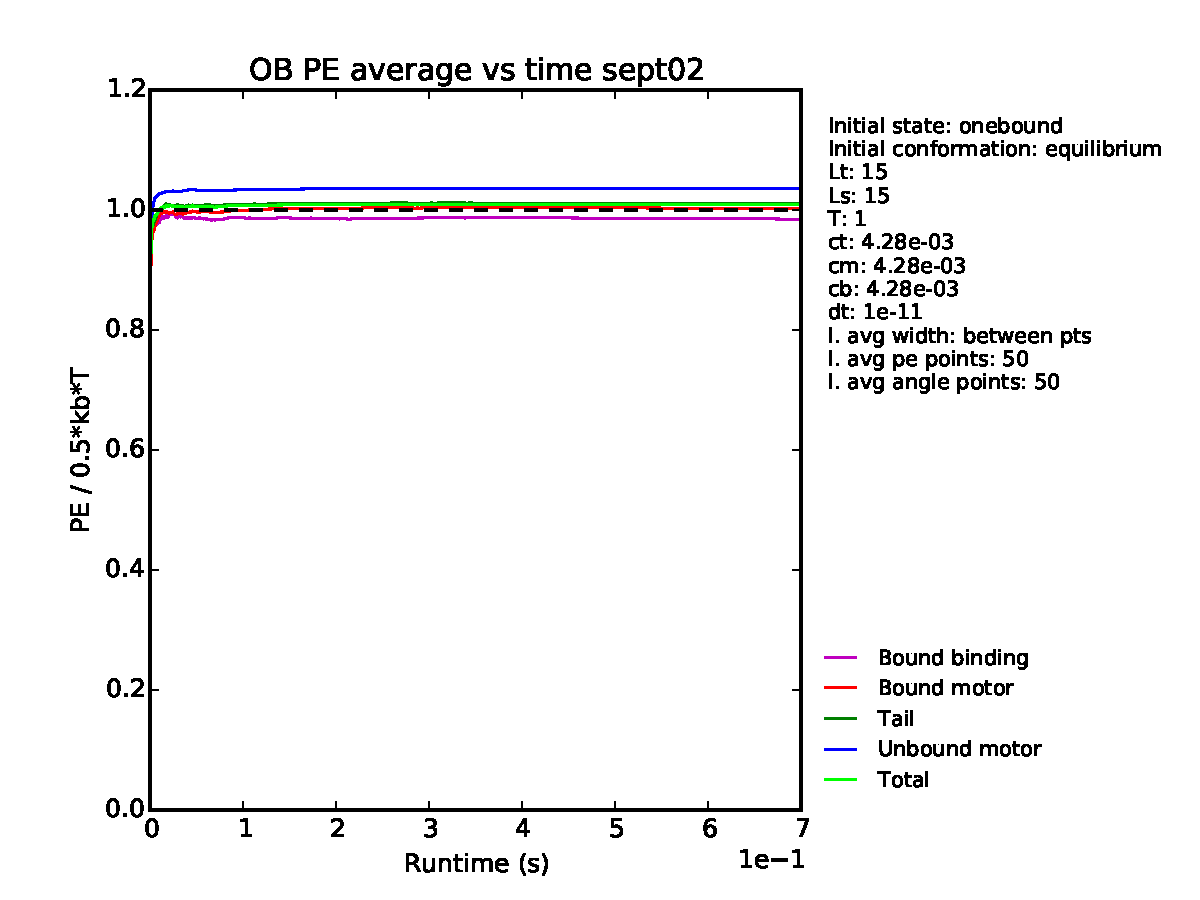
\includegraphics[width=\textwidth]{../figures/OB_Average_PE.pdf}
%%     \caption{Onebound average spring energy.}{Average domain PE of onebound model converging to $\frac12 k_BT$ energy over time.}
%%   \end{minipage}
%%   \hspace{.2cm}
%%   \begin{minipage}[b]{0.45\textwidth}
%%     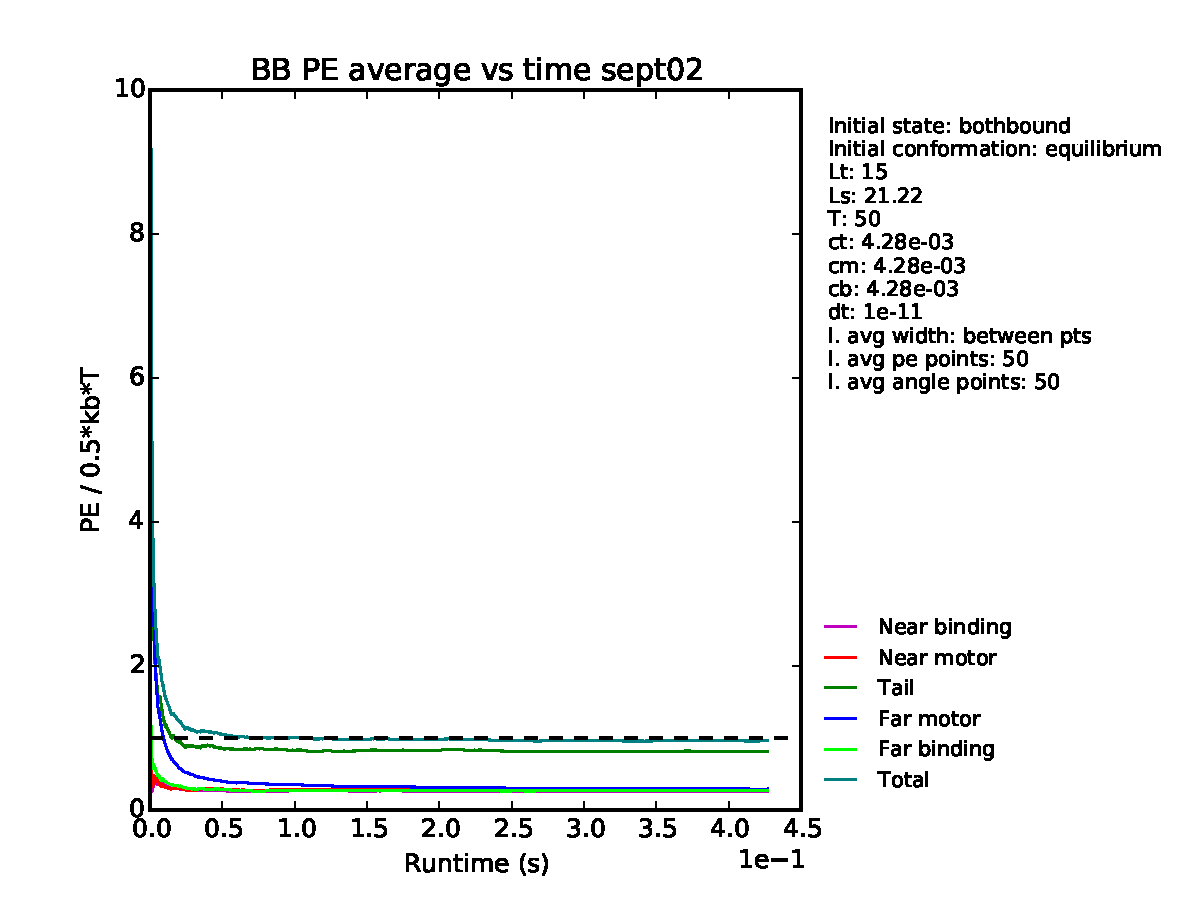
\includegraphics[width=\textwidth]{../figures/BB_Average_PE.pdf}
%%     \caption{Bothbound average spring energy.}{Total domain PE of bothbound model converging to $\frac12 k_BT$ energy over time.}
%%   \end{minipage}
%%   \label{fig:equipartition_agreement}
%% \end{figure}

\section{Model achieves processivity}
When the simulation is run at the parameters shown in (\ref{table:thesis-parameters}), the model exhibits stepping behavior, as shown in Figure (\ref{fig:stepping-trajectory}).\\

\begin{figure}[h]
  \centering
  \begin{tabular}{| l | l | l | l | l | l |}
    \hline
    $k_{b}$ & $k_{ub}$ & $c_b$ &  $c_m$ & $c_t$ & dt\\\hline
    $10^{18} s^{-1}$ & $10^{20} s^{-1}$ & $2.0\Delta G_{ATP}$ & $2.0\Delta G_{ATP}$ & $1.0\Delta G_{ATP}$ & $10^{-10}s$\\ \hline
  \end{tabular}
  \caption{Parameters used in processive simulations.}{These parameters cause processive stepping in the dynein model, as shown in Figures (\ref{fig:stepping-trajectory}) and (\ref{fig:final-histograms}).}
  \label{table:thesis-parameters}
\end{figure}

\begin{figure}[h]
  \centering
  \includegraphics[width=0.9\textwidth]{../../../plots/trajectory-plot_thesis}
  \caption{Dynein simulation displays processive stepping.}{Near and far binding domain x and y projections over the course of several microseconds of simulation. The blue foot corresponds to the ``near'' dimer closer to the viewer, and the red to the far dimer. Top: x-projection of binding domains over time. The motor steps roughly 50nm in 10 $\mu s$. Middle: cartoon depictions of the model during simulation. In the cartoons the blue foot's position on the x-axis corresponds to the time axis on the top and bottom plots. That is, the first cartoon corresponds to dynein at roughly 1 $\mu s$. The first cartoon corresponds to a bothbound model, and the second cartoon corresponds to a onebound model. Bottom: y-projection of binding domains over time. Notice that only one binding domain is above 0nm at any time.}
  \label{fig:stepping-trajectory}
\end{figure}

Figures (\ref{fig:stepping-trajectory}) and (\ref{fig:stepping-trajectory}) demonstrate the model stepping five times, where a step constitutes lifting a binding domain off the microtubule for any amount of time. This behavior indicates that a springy hinge model with shifting equilibrium angles is capable of generating processive stepping behavior. Now that the model has demonstrated stepping behavior, it must be seen if it can generate steps at a size- and time-scale similar to that which real dynein takes in experiment.\\

Another important determination from Figure (\ref{fig:stepping-trajectory}) is the average position of the unbound foot is about 30nm above the microtubule. This is a preliminary finding which may not represent how the model will behave once fit to stepping behavior, so drawing conclusive conclusions from it is impossible. However, it does initially suggest how dynein searches for the microtubule. Instead of hovering near the microtubule looking for a binding site, the motor pulls its foot away from the microtubule, diffusing until pushed downward far enough to bind. This behavior could explain why dynein's stepping pattern is so large: diffusing downward from 30nm would allow significant x-diffusion along the microtubule. This could be contrasted with kinesin, which is smaller and could not move its foot so high off the microtubule.\\

Importantly, the parameters causing processive motion are physically reasonable. The spring constants are roughly the same size as the energy of hydrolysis of ATP, which is reasonable. By a very rough argument, the dynein must move its tail angle by roughly one radian to diffuse enough for a step. This would correspond to a $\Delta G_{spring} = \frac{1}{2}c_t\Delta \theta_t \approx \Delta G_{ATP}$, which is very reasonable. In addition, the tail spring constant is less than the motor and binding spring constants, which is in line with the notion that the tail is much more elastic than the motor or binding domains.\\

\section{Model step size is highly variant}
Figure (\ref{fig:final-histograms}) shows the stepping pattern of the model at the parameters shown in Table (\ref{table:thesis-parameters}). This simulation was run over a much longer time period than that shown in Figure (\ref{fig:stepping-trajectory}), and hence shows much more significant information on the model's stepping behavior.\\

\begin{figure}[H]
  \centering
    \includegraphics[width=0.5\textwidth]{../../../plots/stepping_length_histogram_thesis}%%
    \includegraphics[width=0.5\textwidth]{../figures/weihong-step-size.pdf}
    \caption{Stepping distribution of processive model and experimental dynein.}{Left: step sizes generated by model. Note the model can generate 25nm steps, but has a high preference for <5nm steps. Also note that few backward steps are generated by the model. Simulation run at conditions in (\ref{table:thesis-parameters}). Right: Experimental stepping distribution of dynein, from \cite{weihongpaper}.}
    \label{fig:final-histograms}
\end{figure}

Figure (\ref{fig:final-histograms}) shows the model has a strong preference for $<5$nm steps, but is capable of generating steps up to $25$nm in length, with a fairly even distribution of step frequency between $5$ and $25$nm. This is a very important result, since it indicates that the model is capable of taking a varied step size. This behavior is characteristic of dynein, and hence very important to reproduce.\\

The preference for $<5$nm steps is very un-dynein-like. One explanation is that steps may be defined differently between experimental and modeled dynein. In the simulation, every state transition where the motor unbinds from the microtubule is considered a step and plotted on the stepping histogram. This may not be how the experiment in (\ref{fig:final-histograms}) records steps. Another possibility is that the binding rate used for these simulations is far too high, and thus, immediate rebinding is very likely. A solution may thus be to lower the microtubule binding rate and see if the stepping histogram would level out.\\

The ability of the model to generate near-experiment stepping behavior is imperative if the model is to be considered a proper explanation of dynein's stepping. In the case that changing the binding rate does not remove the small-step preference of the model, it may be necessary to change how the model works. For example, using the total spring-energy-of-binding change to calculate the binding probability may be invalid, or perhaps the entire two-state model will need to be thrown out. The inability of either of these assumptions to predict dynein's behavior would themselves be important findings.\\

Another issue with the simulated histogram is that it shows no steps over $30$nm. This is a problem, since taking $40+$nm steps is characteristic of dynein. Ideally, tuning the parameters of dynein would increase the step size. However, in the case that it can't, this might be an important result. The current model assumes connections between domains are rigid. This may not be a valid assumption, since coiled coils are generally elastic \cite{myosin-cc-elasticity}. Thus it may be necessary to add in elasticity to the model to reproduce long steps.\\

Comparing the simulation results in (\ref{fig:final-histograms}) with the experimental results in (\ref{fig:final-histograms}), it is clear that the model is still far from experimental dynein. However, this is not indicative of a failure of the model, since the simulation parameters have not yet been tuned to dynein. It is very possible that changing the binding rate, unbinding rate and spring constants will change the stepping behavior of the model dramatically. Lowering the binding rate may even out the histogram and prevent instant rebinding. It may also allow the model to diffuse along the microtubule longer, generating longer steps than 25nm. Another issue is the lack of backwards steps, which may also be solved by reducing the spring constants or lowering binding rate.\\

%% \section{Current work: Refining model parameters}
%% Once validated, the model was fit to experimental data. Figure \ref{fig:kb-kub-heatmap} shows a heat map of the behavior of simulations running at many different $k_b$ and $k_{ub}$ values. The color of each point represents the fit quality of a simulation's $\left<t_{ob}\right>$ value to experiment. As can be seen, a good fit is found in the $k_b=XX$, $k_{ub}=YY$ region.

%% \begin{figure}[H]
%%   \centering
%%   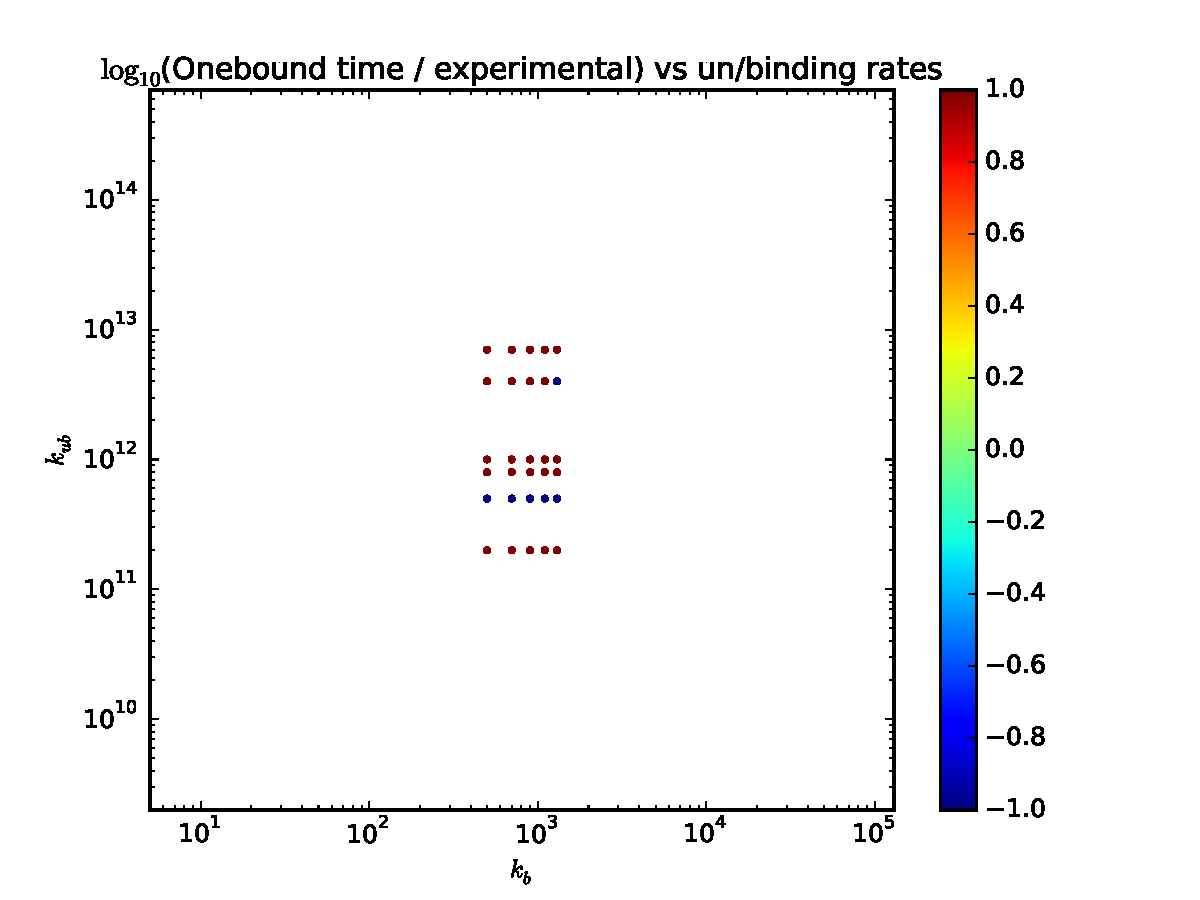
\includegraphics[width=\textwidth]{../figures/kb-kub-contour}
%%   \caption{Heat map comparing $k_b$ and $k_{ub}$ values to time spent in the onebound state. Simulations run for XXXXX seconds at standard conditions shown in Table \ref{table:simulation-std-conditions}, with spring constants $c_b = c_m = c_t = 2.4\Delta G_{ATP}$, $L_s=22.1nm$ and $L_t=11.15nm$. The fit quality of each simulation is decided by $\log_{10}\left(\frac{\left<t_{bb}\right>_{sim}}{\left<t_{bb}\right>_{exp}}\right)$, then fit to the colorbar on the right. Values over or under the colorbar bounds are rounded to the max (1.0 or -1.0).}
%%   \label{fig:kb-kub-heatmap}
%% \end{figure}

\newpage
\chapter{Conclusion}
\label{chap:Conclusion}

%thoughts
%% \textit{It is interesting to note that the hydrolysis of ATP is not actually used to directly power the motor -- binding AMP-PMP, a nonhydrolyzable analog of ATP, can also cause the motor to change from state I to state II \cite{FRETstatepaper}. The specialness of ATP is that it can be broken down into ADP, which causes another conformation change back to state I. Thus, something something the transfer of energy from nucleotide to motor is in its shape, not in its chemistry.}\\

\section{Findings}
The most important findings of this work are that a springy hinge model of dynein can take steps of a similar size to real dynein. What's more, it is likely further tweaking of the model will improve the model's behavior to the point of generating backwards and large steps. This would be a very important result which would strongly support the linker-swing/diffusive-step model of dynein stepping and guide further research.\\

Many studies have been done on dynein, resulting in a large body of literature about the motor's behavior and features. Sifting through this information to find what is important for the motor's step is a difficult task. Mutational studies can remove traits of the motor, deducing what traits are necessary for stepping. However, this process is slow, and it can be difficult to remove large traits of the motor while keeping the engineered dynein representative of the natural motor. This is where simulations come in. Minimal features can be put into a physical model, which can then be tested for behavior similar to real dynein. In this study, we created a mathematical model which simplifies the motor to a rigid hinge structure with harmonic spring energies between the hinges. The equilibrium angles change dynamically to reflect structural changes during dynein's mechanochemical cycle. The model was then subjected to Brownian forces and evolved. If the model generates a stepping pattern similar to real dynein, this would demonstrate that dynein can be thought of as a rigid hinged structure. This would mean that many other traits of dynein may not be vital for stepping, such as stalk elasticity \cite{sarlahmodel}, motor-motor interaction \cite{sarlahmodel}, nucleotide state \cite{cianfroccoreview}, nucleotide state of non-AAA1 nuclease sites \cite{cianfroccoreview}, and changing stiffness of the foot domain \cite{burgess-paper}. Thus future research may want to focus more on linker swing and binding interactions, and less on these other traits.\\

Other findings cast doubt on some aspects of the model. The vast preference of the model for $<5$nm steps suggests that the model may handle binding events unlike real dynein. When binding, the total spring energy of the transition from a onebound to a bothbound state is calculated, then used to calculate the likelihood of transition via a Boltzmann factor. This approach may be overly simple, or take into account the wrong information. It may be that it is necessary to expand the two-state model into a three-state model with a low-microtubule-affinity onebound state immediately after unbinding, to prevent instant rebinding. This state would eventually transition to the high-microtubule-affinity state after some time. If this proves to be necessary to decrease small steps, this would be an interesting result showing that the motor might rely on its low-microtubule-affinity ADP-Pi state to prevent early binding.\\

\section{Further work}
The goal of studying dynein's mechanochemical cycle is to find an explanation for how it work. That is, to find the necessary and sufficient properties of dynein that cause the cycle to happen. Simulations are only part of the recipe for creating a scientific theory. Simulations are easy to implement and can study phenomena which are difficult to design experiments for. However, when experimental data is available, it is generally more reliable than a simulation of the same system. This is because a simulation is only as good as the strength of correspondence between the mathematical model and the system it represents. With dynein, this correspondence can be hard to achieve because the protein is complicated. The model predicts, according to the laws of physics for small objects, how a small machine composed of springy hinges would behave in an aqueous environment. This machine can be made the same size and general shape as dynein, and its conformational angles can be made the same as dynein's, and its state transitions can happen in the same way dynein's do. However, it is never possible to say that this machine ``is'' dynein or represents how dynein actually behaves. Thus, it is only possible to say that the simulation provides sufficient criteria for dynein stepping, not necessary criteria. The simulation shows that the linker-swing/diffusive-step model is sufficient for motion, but it cannot show that this is needed for dynein's walk.\\

\subsection{Experimental validation}
To more strongly support the linker-swing/diffusive step model of dynein motion, more experiments should be done. Demonstrating that dynein requires flexible domain connections in order to take such broad steps would be one powerful experiment. Mutating the foot and tail domains to be more rigid, then examining stepping behavior would be one way to see if rigidity is necessary for random steps. Another experiment could use FRET (Forster Resonance Energy Transfer) and fluorophores on the microtubule and foot domain to track how the distance between the two regions evolves with time. This could provide information about the average distance between the MTBD and MT, which would validate this work's finding that the MTBD mostly hovers. More importantly, FRET data could be fit to models to predict the amount of diffusion the foot domain undergoes over the course of a step. Significant diffusion would indicate that diffusion may be very important for the step. Experiments with both feet labeled could get similarly good information.\\

%% \textbf{Talk to Dr. Hsu about this sort of thing...what experiments could be used to validate the model?}

\subsection{Further questions}
If the model were validated by FRET and rigidity mutation studies, there are many other interesting things which could be found from it. First, the amount of work done by the motor could be found by inducing an artificial drag force pulling the protein's motor domains against its direction of travel. This force could be integrated over dynein's trajectory to find the work the model exerted on its artificial cargo. This could be used to estimate the efficiency of the motor. Another interesting study would be to add binding sites to the model, only allowing it to bind at $\alpha-\beta$ tubulin dimerization sites, like real dynein. This would mandate re-fitting the binding constants to the new environment. It would be interesting to know if this model behaves more, or less dynein-like than the original. This would help answer the question of whether dynein searches for a binding site on the microtubule, or if it is naturally tuned to bind at the right site.\\

Another very interesting simulation which could be run could help answer the open question of why kinesin and dynein, though using similar mechanisms, produce such different steps. Kinesin, unlike dynein, conducts all of its chemistry directly on its foot. This translates to effectively having two fewer joints than dynein. Kinesin's stroke is believed to involves a similar foot unbinding, kicking forward, rebinding, then lurching the motor forward mechanism. The dynein model could be used to construct a very rough model of kinesin by shrinking the tail linkers and increasing the motor domain spring constant $c_m$ high enough to simulate a rigid hinge. This model could then be reduced to the size of kinesin, given the proper equilibrium angles, and simulated with Brownian dynamics. If this new model even roughly manages to mimic experimental kinesin stepping, that would be fascinating. This result would show that the differences between kinesin and dynein can be explained exclusively through the values of spring constants $c_t$, $c_m$, $c_b$, lengths $L_s$ and $L_t$, equilibrium angles and un/binding constants. This would mean the differences between the two motors are primarily due to the conformational angles the motors take with the microtubule and between their own domains, not because of differences in their mechanism.\\

\subsection{The future of dynein research}
The motor protein field has come a long way over the past two decades. Theoretical papers in the 90s, such as \textit{Bhaba et. al.} \cite{bhabha-paper},  opened up many questions about how cells can use proteins and simple chemical reactions to generate directed, finely-controlled motion. Following these papers came low-resolution structures and experiments testing the stepping behavior, directionality, conformation changes and chemical affinities of these motors. As structural technology got better, resolution got better, until eventually amino-acid resolution structures were found~\cite{schmidt-carter}. These structures allowed more informed hypotheses to integrate experimental data and structures into well-advised theories on motor motility, such as \textit{Andreasson et. al.} for kinesin~\cite{kinesin-cycle} and \textit{Cianfrocco et. al.} for dynein \cite{cianfroccoreview}. These theories are now being tested using state of the art methods. For example, a lab at Penn State is currently exploring kinesin dynamics using gold nanoparticles, and is capable of getting 2nm spatial resolution and 1ms temporal resolution~\cite{kinesin-gold-nanoparticle}. This level of detail would provide intra-step information about the kinesin mechanochemical cycle, confirming or rejecting hypotheses about how the motor steps. If such technology were applied to dynein, the accuracy of the Cianfrocco model and the role of diffusion would be definitively determined. However, such experiments take time to design and implement. In the meantime, modelling projects like the one in this thesis can be used to provide rough windows into the nanoscale world, guiding future experimental work. They sanity-check theories and help scientists form new questions, such as if dynein drags along the microtubule or diffuses above it. It is uncertain what direction the field will go over the coming decade, but it is clear that now is a very exciting time for dynein research.\\

%----------------------------------------------------------------------------------------
%	THESIS CONTENT - APPENDICES
%----------------------------------------------------------------------------------------

\appendix % Cue to tell LaTeX that the following "chapters" are Appendices

% Include the appendices of the thesis as separate files from the Appendices folder
% Uncomment the lines as you write the Appendices

\allowdisplaybreaks

\chapter{Onebound equations} % Main appendix title
\label{sec:AppendixOneboundEquations}

The following is a continuation of the derivation for the full motion equations used to time evolve the onebound model:

\begin{align*}
AA &= L_s\sin\theta_{bb}      &   LL &= -L_s\cos(\theta_{bb})\\
BB &= L_t\sin(\theta_{bm})    &	 MM &= -L_t\cos(\theta_{bm})\\
CC &= -L_t\sin(\theta_{um})   &	 NN &= L_t\cos(\theta_{um})\\
DD &= -L_s\sin(\theta_{ub})   &	 OO &= L_s\cos(\theta_{ub})\\
\\
EE &= -\gamma_m (X_{bm} - X_{bb})       &  PP &= -\gamma_m (Y_{bm} - Y_{bb})\\
FF &= \gamma_m (X_{t } - X_{bm})        &	 QQ &= \gamma_m (Y_{t } - Y_{bm})\\ 
GG &= -\gamma_t (X_{t } - X_{bm})       &	 RR &= -\gamma_t (Y_{t } - Y_{bm})\\
HH &= \gamma_t (X_{um} - X_{t })        &	 SS &= \gamma_t (Y_{um} - Y_{t })\\ 
II &= -\gamma_m (X_{um} - X_{t })       &	 TT &= -\gamma_m (Y_{um} - Y_{t })\\
JJ &= \gamma_m (X_{ub} - X_{um})        &	 UU &= \gamma_m (Y_{ub} - Y_{um})\\ 
KK &= -\gamma_b (X_{ub} - X_{um})       &	 VV &= -\gamma_b (Y_{ub} - Y_{um})\\
\end{align*}%
%
\[
\begin{pmatrix}
  AA & 0 & 0 & 0 & EE & FF & 0 & 0\\
  AA & BB & 0 & 0 & 0 & GG & HH & 0\\
  AA & BB & CC & 0 & 0 & 0 & II & JJ\\
  AA & BB & CC & DD & 0 & 0 & 0 & KK\\
  LL & 0 & 0 & 0 & PP & QQ & 0 & 0\\
  LL & MM & 0 & 0 & 0 & RR & SS & 0\\
  LL & MM & NN & 0 & 0 & 0 & TT & UU\\
  LL & MM & NN & OO & 0 & 0 & 0 & VV\\
\end{pmatrix}
\begin{pmatrix}
    \dot{\theta}_{bb}\\
    \dot{\theta}_{bm}\\
    \dot{\theta}_{um}\\
    \dot{\theta}_{ub}\\
    \lambda_{bs}\\
    \lambda_{bt}\\
    \lambda_{ut}\\
    \lambda_{us}\\
  \end{pmatrix}
=
  \begin{pmatrix}
    -F_{bmx} + \gamma_m R_{bmx}\\
    -F_{tx} + \gamma_t R_{tx}\\
    -F_{umx} + \gamma_m R_{umx}\\
    -F_{ubx} + \gamma_b R_{ubx}\\
    -F_{bmy} + \gamma_m R_{bmy}\\
    -F_{ty} + \gamma_t R_{ty}\\
    -F_{umy} + \gamma_m R_{umy}\\
    -F_{uby} + \gamma_b R_{uby}\\
  \end{pmatrix}
\]

Solving the above system for $\dot{\theta}_{bb}, \dot{\theta}_{bm}, \dot{\theta}_{um}$ and $\dot{\theta}_{ub}$ gives the desired velocities. Solution was done via Mathematica.

\chapter{Bothbound equations} % Main appendix title
\label{sec:AppendixBothboundEquations}

The following are the full motion equations used to time evolve the bothbound model:

\begin{center}
  \begin{minipage}{0.3\textwidth}
    \begin{align*}
      a &= \frac{-dXnm}{dLn}\\
       b &= \frac{-dXnm}{dLf}\\
       c &= -(x_{nm} - x_{nb}) / \gamma_m\\
       d &= (x_t - x_{nm}) / \gamma_m\\
       e &= \frac{-dXt}{dLn}\\
       f &= \frac{-dXt}{dLf}\\
       g &= -(x_t - x_{nm}) / \gamma_t\\
       h &= (x_{fm} - x_t) / \gamma_t\\
       i &= \frac{-dXfm}{dLn}\\
       j &= \frac{-dXfm}{dLf}\\
       k &= -(x_{fm} - x_t) / \gamma_m\\
       l &= (x_{fb} - x_{fm}) / \gamma_m\\
    \end{align*}
  \end{minipage}
  \begin{minipage}{0.3\textwidth}
    \begin{align*}
       m &= \frac{-dYnm}{dLn}\\
       n &= \frac{-dYnm}{dLf}\\
       p &= -(y_{nm} - y_{nb}) / \gamma_m\\
       q &= (y_t - y_{nm}) / \gamma_m\\
       r &= \frac{-dYt}{dLn}\\
       s &= \frac{-dYt}{dLf}\\
       t &= -(y_t - y_{nm}) / \gamma_t\\
       u &= (y_{fm} - y_t) / \gamma_t\\
       v &= \frac{-dYfm}{dLn}\\
       w &= \frac{-dYfm}{dLf}\\
       x &= -(y_{fm} - y_t) / \gamma_m\\
       y &= (y_{fb} - y_{fm}) / \gamma_m
    \end{align*}
  \end{minipage}
\end{center}
%
\[
\begin{pmatrix}
  a & b & c & d & 0 & 0\\
  e & f & 0 & g & h & 0\\
  i & j & 0 & 0 & k & l\\
  m & n & p & q & 0 & 0\\
  r & s & 0 & t & u & 0\\
  v & w & 0 & 0 & x & y\\
\end{pmatrix}
\begin{pmatrix}
    \dot{L}_{n}\\
    \dot{L}_{f}\\
    \lambda_{ns}\\
    \lambda_{nt}\\
    \lambda_{ft}\\
    \lambda_{fs}\\
  \end{pmatrix}
=
\begin{pmatrix}
  -\frac{1}{\gamma}F_{nmx} - R_{nmx}\\
  -\frac{1}{\gamma}F_{tx}  - R_{tx}\\
  -\frac{1}{\gamma}F_{fmx} - R_{fmx}\\
  -\frac{1}{\gamma}F_{nmy} - R_{nmy}\\
  -\frac{1}{\gamma}F_{ty}  - R_{ty}\\
  -\frac{1}{\gamma}F_{fmy} - R_{fmy}\\
\end{pmatrix}
\]

Solving the above system for $\dot{\theta}_{nm}$ and $\dot{\theta}_{fm}$ gives the desired velocities. Solution was done via Mathematica.

\chapter{Conformational tests}
\label{sec:conformational-tests}
The models were tested in the following different conformations to verify they behaved as expected:\\

\textbf{Onebound tests}
\begin{itemize}
\item \textbf{Onebound:} \textit{Upwards line conformation with no forces.} Check that all domain x-values are zero$^*$ and all y-values are the proper addition of $L_s$ and $L_t$ lengths. Also checks that all angular velocities are zero. This test verifies that the angle scheme is defined properly, that the model can handle straight lines without generating NaNs and that there are no velocities (angular or Cartesian) without forces.
\item \textbf{Onebound:} \textit{Horizontal line conformation with no forces.} Check that all domain y-values are zero and all x-values are the proper addition of $L_s$ and $L_t$ lengths. Also check that all velocities are zero. This test double-verifies that the coordinate system behaves as expected and that velocities are zero in the absence of forces.
\item \textbf{Onebound:} \textit{Upwards line conformation with +x forces} Check that Cartesian x-velocities are positive and y-velocities are zero. Verifies that the Cartesian velocities have the expected sign.
\item \textbf{Onebound:} \textit{Upwards line conformation with +y forces} Check that all Cartesian velocities are zero. Verifies that upwards forces in an already-vertical stalk have no effect on velocity.
  \item \textbf{Onebound:} \textit{Prepowerstroke opposing internal/brownian forces} Check that, for two onebound models, one with +x spring forces and no Brownian forces and the other with -x Brownian forces and no spring forces, that the velocities of each unbound domain are equal and opposite. Verifies that equal Brownian and internal forces have the same magnitude and direction of effect on velocities.
\end{itemize}

These checks for equality are within a margin of error of $\epsilon = 1e^{-5}$.\\

These tests together verify that the onebound model's internal coordinate system's directions match the XY coordinate system directions, that the angular directions in the model properly align with the $\pm x$ and $\pm y$ directions of the XY coordinate system, that velocities have the proper magnitude at zero force and proper sign at nonzero force, and that Brownian and internal forces are in the same unit system. There are still errors which could exist in the model pertaining to magnitude of velocity, which will be tested for in the energy conservation section.\\

\textbf{Bothbound tests}
\begin{itemize}
\item \textbf{Bothbound:} \textit{Upwards line conformation with no Brownian forces.} Both MTB domains are very close together ($L=10^{-25}$) and motor domains nearly vertical ($\theta_{n/f} = \pi \pm 10^{-15}$). Equilibrium angles set to have a vertical line as the lowest energy point. Checks that domain x-values are zero$^*$, domain y-values are the correct combination of $L_s$ and $L_t$ lengths, all angles are at equilibrium and all forces are zero. Verifies that the domains are properly oriented by the angles, the angles are defined properly and forces are calculated from angles properly.
\item \textbf{Bothbound:} \textit{Equilateral house conformation with outward x-forces.} The model forms the shape of a square with an equilateral triangle on top, with the tail domain as the triangle. Checks if all domains are at the desired locations and the derivatives are the proper sign and are equal and opposite to their counterparts on the opposing side of the house. This test verifies that the angular system behaves as expected and forces are symmetric about the two dimers.
\item \textbf{Bothbound:} \textit{Two table conformations with near/far domains flipped.} Two models are put in the same table-like conformation, but the near/far domains are flipped. Checks if opposite domains have the same positions and forces. Re-verifies that the model is symmetric in position and force between the two dimers.
\end{itemize}

These tests verify the bothbound model's angle system behaves as expected, forces are zero when expected and have the proper signs, and that the whole system is symmetric with either dimer.

%----------------------------------------------------------------------------------------
%	BIBLIOGRAPHY
%----------------------------------------------------------------------------------------

\printbibliography[heading=bibintoc]

%----------------------------------------------------------------------------------------

\end{document}  
